%\documentclass[letter]{article}
\documentclass[letter,12pt]{article}
\usepackage[letterpaper,right=1in,left=1in,top=1in,bottom=1in]{geometry}

\usepackage{hyperref}
\usepackage{url}
\usepackage[pdftex]{graphicx}
\usepackage[longnamesfirst, sort]{natbib}\bibpunct[]{(}{)}{,}{a}{}{;}
\usepackage{arydshln}
\usepackage{amsmath}

%\usepackage{rotating}
%\usepackage{pdflscape}

\newcommand{\mc}{\multicolumn}

\graphicspath{{../graphs/}}
%\graphicspath{{graphs/}}

\begin{document}

\title{The Effects of Automated Redistricting and Partisan Strategic Interaction on Representation: \\ 
       The Case of Mexico\thanks{Paper prepared for delivery at the Annual Meeting of the American Political Science Association, Washington, DC, August 2014. We thank the Federal Electoral Institute (IFE) and the Federal Voter Registry (RFE). Special thanks to IFE's Cartography Department for sharing their experience with automated redistricting since 1996 and most of the data we analyze. We also acknowledge the support from the Asociaci\'on Mexicana de Cultura A.C.\ and CONACYT for this work.}}
\author{Micah Altman {\small \url{escience@mit.edu}} \\
        Eric Magar {\small \url{emagar@itam.mx}} \\
        Michael McDonald {\small \url{michael.mcdonald@ufl.edu}} \\  %\\ University of Florida, Gainesville\\
        Alejandro Trelles {\small \url{lat44@pitt.edu}}
      }
\date{\today}
\maketitle


\begin{abstract}
%Abstract Version 1
\noindent In the U.S.\ redistricting is deeply politicized and often synonymous with gerrymandering ---the manipulation of boundaries to promote the goals of parties, incumbents, and racial groups. In contrast, Mexico’s federal redistricting has been implemented nationwide since 1996 through automated algorithms devised by the electoral management body (EMB) in consultation with political parties. In this setting, parties interact strategically and generate counterproposals to the algorithmically generated plans in a closed-door process that is not revealed outside the bureaucracy. Applying geospatial statistics and large-scale optimization to a novel dataset that has never been available outside of the EMB, we analyze the effects of automated redistricting and partisan strategic interaction on representation. Our dataset comprises the entire set of plans generated by the automated algorithm, as well as all the counterproposals made by each political party during the 2013 redistricting process. Additionally, we inspect the 2006 map with new data and two proposals to replace it towards 2015 in search for partisan effects and political distortions. Our analysis offers a unique insight into the internal workings of a purportedly autonomous EMB and the partisan effects of automated redistricting on representation.

% Comment [Eric and Alejandro]: Two alternative abstract versions bellow.
% Comment [Alejandro]: Given the direction the paper is taking, I wrote a new abstract and moved the previous version to option 3. The floor is open for comments, suggestions or modifications...

% Abstract Version 2:
% Mexico’s federal redistricting has been implemented nationwide since 1996 through automated algorithms devised by the electoral management body (EMB) in consultation with political parties. In this setting, parties interact strategically and generate counterproposals to plans in a closed-door process that is not revealed outside the bureaucracy.The way that redistricting has played out so far in Mexico raises a number of questions: Were the adopted redistricting criteria politically neutral? Were the plans produced algorithmically, in fact, optimal with respect to the selected criteria? How did partisan counterproposals differ from the bureaucratic solution? What influence did parties have on the final proposed plan? Can automated and partisan interactive  models  generate relatively fair and unbiased plans? We address these questions by applying geospatial statistics and large scale optimization to a novel dataset that comprises the entire set of plans generated by the automation algorithm and all plans proposed by political parties during the 2013 redistricting process. Our findings offer a unique insight into the internal workings of a purportedly autonomous EMB and the partisan effects of automated redistricting on representation.

%Abstract Version 3:
%In the U.S. redistricting is deeply politicized and often synonymous with gerrymandering ---the manipulation of boundaries to promote the goals of parties, incumbents, and racial groups. In contrast, starting in 1996, Mexico's federal redistricting has been implemented nationwide through an automated algorithm devised by the electoral management body (EMB) in consultation with political parties. The system purports to produce plans that are optimal. However, until recently, Mexico’s redistricting process has been closed to both public participation and inspection. We inspect new data of the 2006 map and two proposals to replace it towards 2015 in search for partisan effects and political distortions. Unlike analysis of the votes-to-seats conversion at the national-level, state-level data reveal no evidence of systematic party bias. What bias there is in federal districts is of another kind, a big bonus for larger parties (or vote responsiveness) typical of plurality rule in single-member districts. Since most states distribute few seats each, the large party bonus of states' federal districts doubles the estimate with national data. Since the PRI is the largest party in most states, it receives a substantial seat bonus.

% Comment [Micah]: Last two sentences of version 3 are unclear. Reword? 
\end{abstract}

% Comment [Eric]: Possible argument for the presentation.
% Expert committees can remove partisan bias from redistricting.
% Mexico's process allows parties to respond. Offers leverage to infer party preferences and degree of influence. 
% Analysis of party bias and responsiveness informs this, directly. 

Redistricting is political. Map drawers in the US have long been suspected of distorting representation to protect incumbents from competition \citep{mayhew1974vanishingMg,cox.katz.2002,erikson1972malapportionment,engstrom2006redisttrictApsr,mcdonald.CommVsLegisRedistrict2004}. Seeking to rid the process of gerrymandering, a small but growing proportion of state governments, in charge of congressional redistricting in the US, have delegated this authority to experts. Mexican parties do the same since 1996. Federal Electoral Institute personnel use self-taylored, automated algorithms to propose a map deemed optimal. The parties react by offering counterproposals. We verify the extent to which technocrats have replaced politics \citep{lujambio.vives.2008} by inspecting new Mexican data. Our work sheds light on redistricting by independent boards. 

Independent boards and the electoral systems under which they operate are never neutral \citep{lijphart.1990,rossiter.etal.1997,estevez.magar.rosas.2008} despite IFE's claims to the contrary. Rather than expunging bias altogether, experts replace one sort with another. Many opportunities for manipulation and distorsion remain despite automation. In particular, IFE has redistricted behind closed doors, without public scrutiny, much less participation \citep{trelles.mtz.tesisItam.2007}. The scant information reaching the media is insufficient to validate the new map before it is adopted. 

The 2010 census data were unavailable in time to adjust federal districts before the 2012 general election. The process begun one year later but coincided with a major overhaul of the election regulator. Parties postponed the adoption of a plan that was ready. We assess this plan in seach for effects in representation. We inspect data that never before been available outside of the Mexican government. It comprises the entire map that was machine generated, and two rounds of counterproposals by political parties. Analysis offers a unique insight into the politics of redistricting.

The paper proceeds thus...

The focus of analysis are single-member district (SMD) seats in the federal chamber of deputies. The compensatory, proportional representation (PR) seats, untouched by the redistricting proposal, are removed from the picture. 

\section{Redistricting by an independent board}

Mexico adopted a mixed member electoral system for the lower house of Congress in 1979. Three hundred single-member districts were drawn to elect two-fifths of the chamber by plurality rule. Districts were not redrawn until 1997, coinciding with the first free and fair election. A second redistricting process took place in 2006, and a third towards 2015. The latter was finalized but never adopted. We refer to district maps by the first year they were in use, not by the actual year they were drawn.\footnote{The maps were actually finalizedin 1977, 1996, 2005, and 2013.} Redistricting since 1997 is automated and in consulation with political parties in a process involving three steps \citep{lujambio.vives.2008,trelles.mtz.tesisItam.2007}. 

As in the U.S., no district crosses state boundaries. Redistricting therefore starts with the apportionment of congressional seats to the 31 states and the Federal District according to population. The next section discusses the method. In contrast to the U.S. \citep{szpiro.numbersRule.2010}, little, if any debate about alternative apportionment methods has been undertaken. 

Next, a heuristic optimization model to aggregate congressional districts from states' \emph{electoral sections} is devised. Sections are geo-statistical units, similar to the U.S.\ census tracts. Median section population in the 2010 census was 1,280 inhabitants, with a maximum at 79,232. Mexico's surface is covered by more than 66 thousand sections. Heursitics have been refined with every redistricting round. That used for 2015 prepared districts that must be contiguous and not partition municipalities with sizeable indigenous populations. The heuristic rewards population balance (within limits to be discussed), district compactness, the preservation of municipal boundaries, and the minimization of district travelling times. A map maximizing the heuristic is proposed. Towards the 2015 redistricting, a proposal was presented on July 17, 2013 for discussion. 

\begin{table}
\begin{center}
  \begin{tabular}{lrrr|rrr|r}
    Party & national & state  & total 1st & national& state  & total 2nd & Total \\ \hline
    PAN	  & 17/22    & 2/20   & 19/42     & 17/24   & 4/16   & 21/40     & 40/82 \\
    PRI	  & 0/0      & 2/28   & 2/28      & 8/30    & 6/26   & 14/56     & 16/84 \\
    PRD	  & 3/27     & 2/21   & 5/48      & 5/29    & 5/18   & 10/47     & 15/95 \\
    PT	  & 1/12     & 1/20   & 2/32      & 3/15    & 1/16   & 4/31      & 6/63 \\
    PVEM  & 0/0      & 1/20   & 1/20      & 7/28    & 3/17   & 10/45     & 11/65 \\
    MC    & 1/17     & 0/21   & 1/38      & 6/32    & 2/16   & 8/48      & 9/86 \\
    PNA   & 0/1      & 1/18   & 1/19      & 4/11    & 3/17   & 7/28      & 8/47 \\
    IFE   & 0/0      & 1/9    & 1/9       & 0/0     & 5/13   & 5/13      & 6/22 \\ \hline
    Total & 22/79    & 10/157 & 32/236    & 50/169  & 29/139 & 43/308    & 111/544 \\
  \end{tabular}
  \caption{Counterproposals to the first and second proposals at the National and Local Surveilance Committees. Denominator reports the number of counterproposals made, numerator how many were adopted. Prepared by authors with information from the Federal Electoral Institute.}\label{T:counterprops}
\end{center}
\end{table}
 
Last, parties make observations to the map and change district boundaries. Counterproposals failing to meet the general criteria are discarded. If more than one counterproposal to a district is made, all not maximizing the heuristic are dropped. Two rounds of complaints/revisions took place in preparation for the 2015 map, which table \ref{T:counterprops} summarizes. Parties were quite active in challenging proposed districts, making 75 counterproposals each on average. PAN was by far the most successfull, getting nearly half of 82 proposals accepted, compared to about one-fifth for other major parties. Amendments originated in both national (at the National Surveilance Committee) and state parties (at 32 Local Surveilance Committees). The complaint/revision stage improved in some respects over the years. Towards 2015, an organizational map-sharing tool was adopted, which standardized counterproposals while letting parties see each other's complaints and amendements---likely adding a strategic dimension. Counterproposals to the 2015 map received by the redistricting technical committee surged. A total of 544 counterproposals were made towards 2015, more than twice towards 1997 and 2006. The breakdown consists of 236 counterproposals made to IFE's first proposal, 157 from the local parties and 79 from national parties; and 308 made to the second proposal, 139 by local and 169 by national parties. The final proposal for Council General approval was presented on October 15, 2013. The Council chose not to decide before the end of the month. The 2015 midterm election, it was soon after learned, will be held with outdated districts. 

In another, key respect, all processes have remained opaque activities between electoral regulators and party representatives. New technology letting anyone interested, with little more than an internet connection, see proposals, react, and improve them through crowsourcing \citep{altman.mcdonald2011bard}, remains to be adopted. 

\section{Malapportionment I: states in Congress}

The Hamilton method of largest remainders is used for apportionment to the states \citep[][:10]{balinskiYoung2001FairRep}. The quota $Q$ (or price) of a seat is the nation's population divided by 300, the number of seats since 1979. A first allocation is made by dividing each state's population by $Q$, rounded down. Unallocated seats, if any, are awarded to states with largest fractional remainders. 

\begin{figure}
\begin{center}
  \begin{tabular}{cc}
    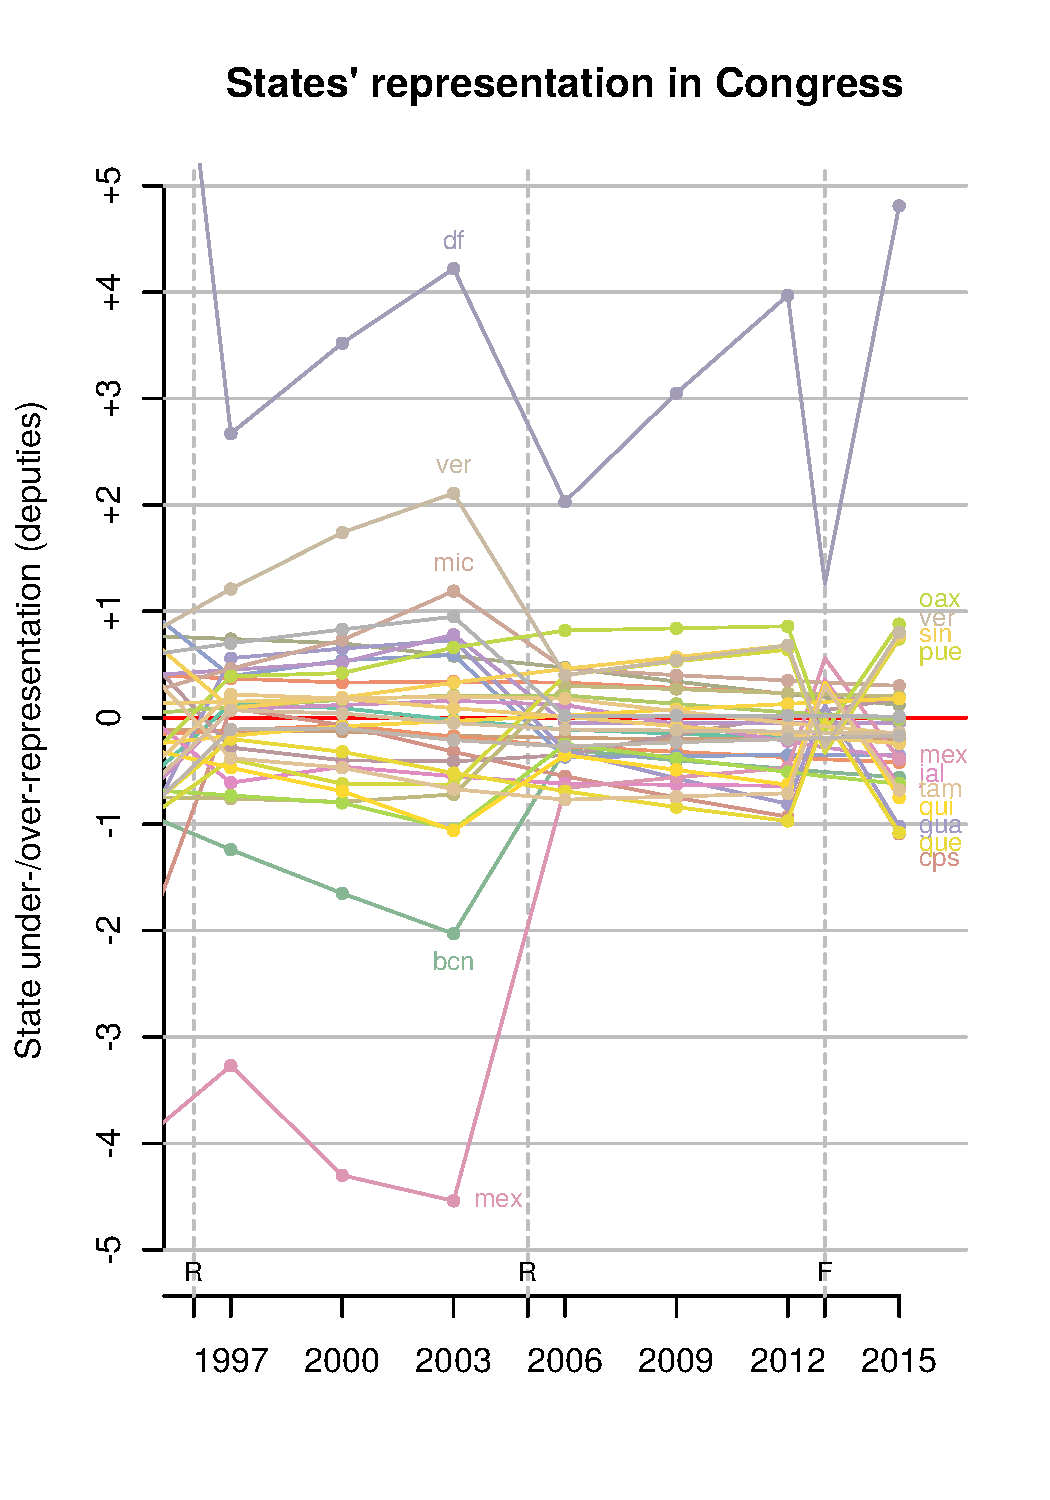
\includegraphics[width=.5\columnwidth]{statesUnderOverRep.pdf} & 
    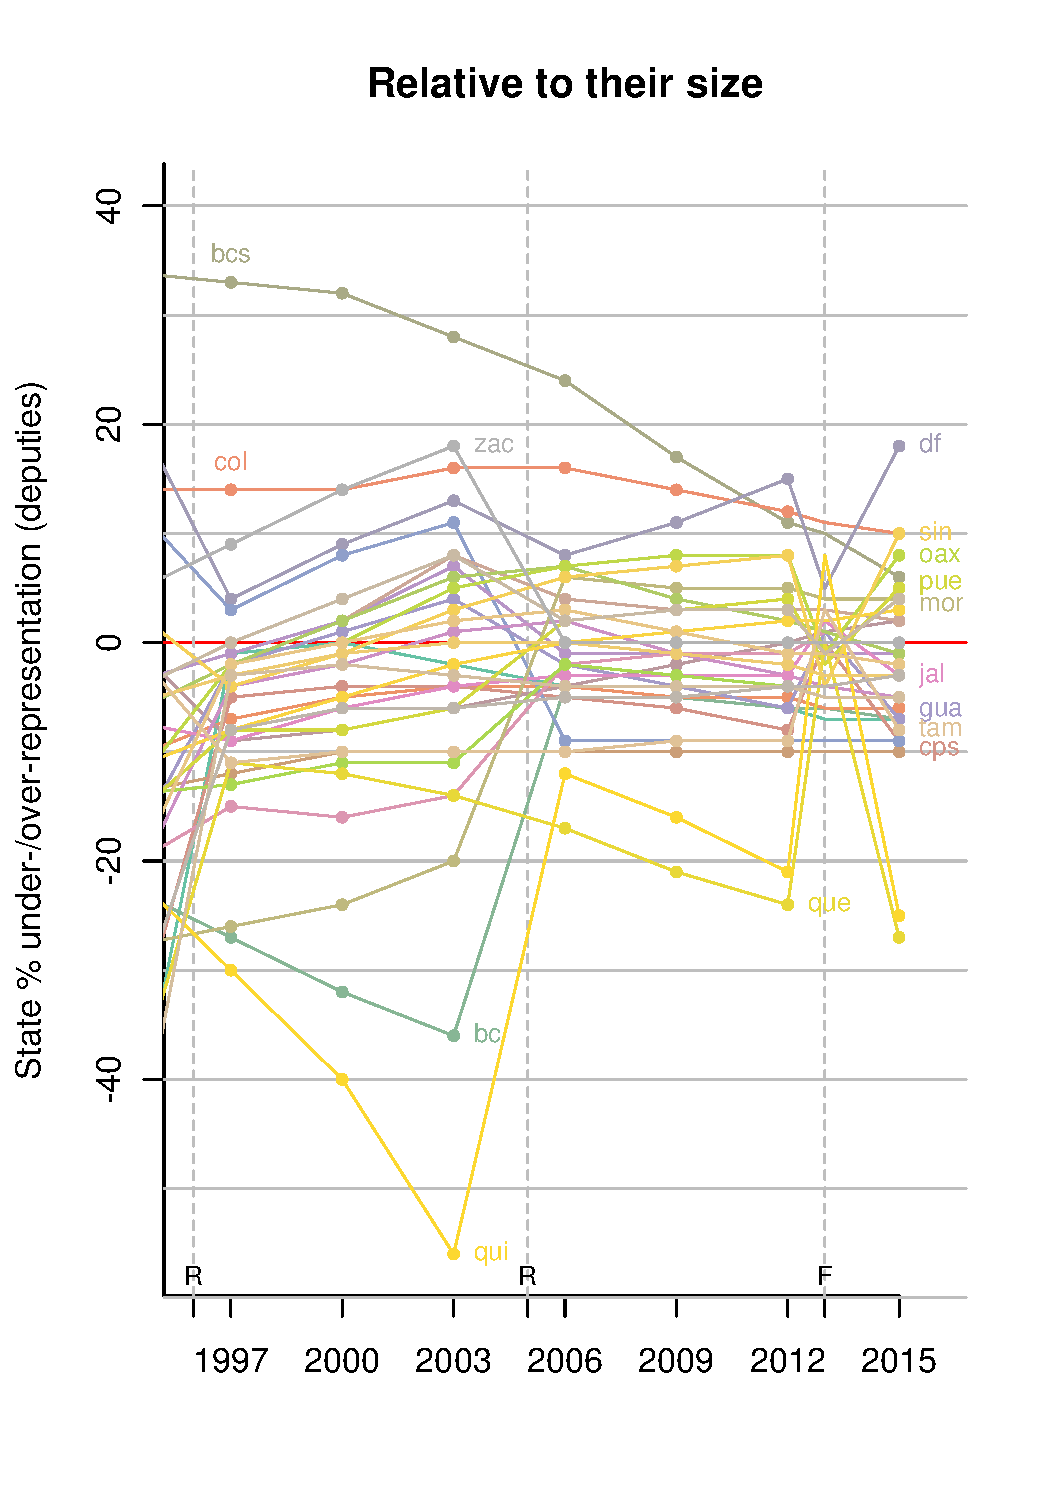
\includegraphics[width=.5\columnwidth]{statesUnderOverRep-rel.pdf} \\ 
  \end{tabular}
  \caption{Demography and state apportionment. Lines connect the lower chamber seats aportioned to seats due difference for each state over time. Letters R in the horizontal axis indicate redistricting, letter F a failed redistricting attempt (reporting the effect it would have had).}\label{F:underOverRep}
\end{center}
\end{figure}

Figure \ref{F:underOverRep} summarizes state's representation in Congress. Over- and under-representation vis-\`a-vis demography is one form of malapportionment that few electoral systems can render negligible. Mexico's does not. Population from the 1995 and 2005 partial, and the 2000 and 2010 general censi was interpolated linearly to show this. The measure is the seats apportioned to seats due difference (positives indicate over-representation). Since the first term of the measure is an integer but the second a real number, a fraction is bound to remain. Fractions in well-apportioned systems should all less than 1 in absolute value. The left panel of Figure \ref{F:underOverRep} shows that this is mostly the case for Mexico, but exceptions are systematic. 

It is also plain that redistricting towards 2006 corrected, to some extent, important distorsions that redistricting towards 1997 had failed to wipe. Under-representation of Baja California, but especially of the Mexico State dropped respectively from two and five deputies less than due (deficits of 30 percent and less than 10 in relative terms), respectively. Over-represented Veracruz behaved near symmetrically to Baja in absolute terms (not relative). And a distorsion strongly favoring the Federal District ($+4$ deputies) was somewhat attenuated towards the 2006 election, but never removed. Relative over-representation is substantial for the smallest states---entitled to two seats at leastlike all states, which Southern Baja California and Colima weren't really worth demographically until quite recently---migrant-worker-exporter Zacatecas up to 2003, and the Federal District of late. With this brief description, it is puzzling that the redistributive nature of apportionment has not pushed for the adoption of alternative methods. The seventeen states that were under-representedin 2006 jointly controlled a majority (162) of single-member districts; fouteen of them have always been below the red line indicating fair representation. 

Whether distrisions are purely mechanical, caused by difficulties to estimate population growth accurately, or purposeful remains an open question. But analysis should be able to detect whether or not this distorsion is a source of bias in the translation of votes to seats. 

Not sure if this is useful anymore... I thought we might discuss what failed redistricting for 2015 would have done. 

\begin{tabular}{l|c|c|}
                  & \mc{2}{c}{Would 2013 have reverted?}\\ \cline{2-3}
State is          & yes                  & no \\ \hline
over-represented  & df oax pue sin       & bcs col\\ \hline
under-represented &  cps gua que qui tam & ags bc cam coa dgo\\ \hline
                  &                      & cua gue hgo mic mor  \\ 
on target         & jal mex ver          & nay nl san son tab  \\ 
                  &                      & tla yuc zac \\ \hline
\end{tabular}

\section{Malapportionment II: against one person, one vote}

Despite automation and transparent redistricting criteria, Mexican parties in general, and IFE in particular, have been remarkably tolerant to unequally sized districts---another form of malapportionment. It is related in some degree to the distorsion last discussed because differences in state apportionment perforce create size differences \emph{across} states. But size inequality \emph{within} states is also observed and substantial. 

\begin{figure}
\begin{center}
    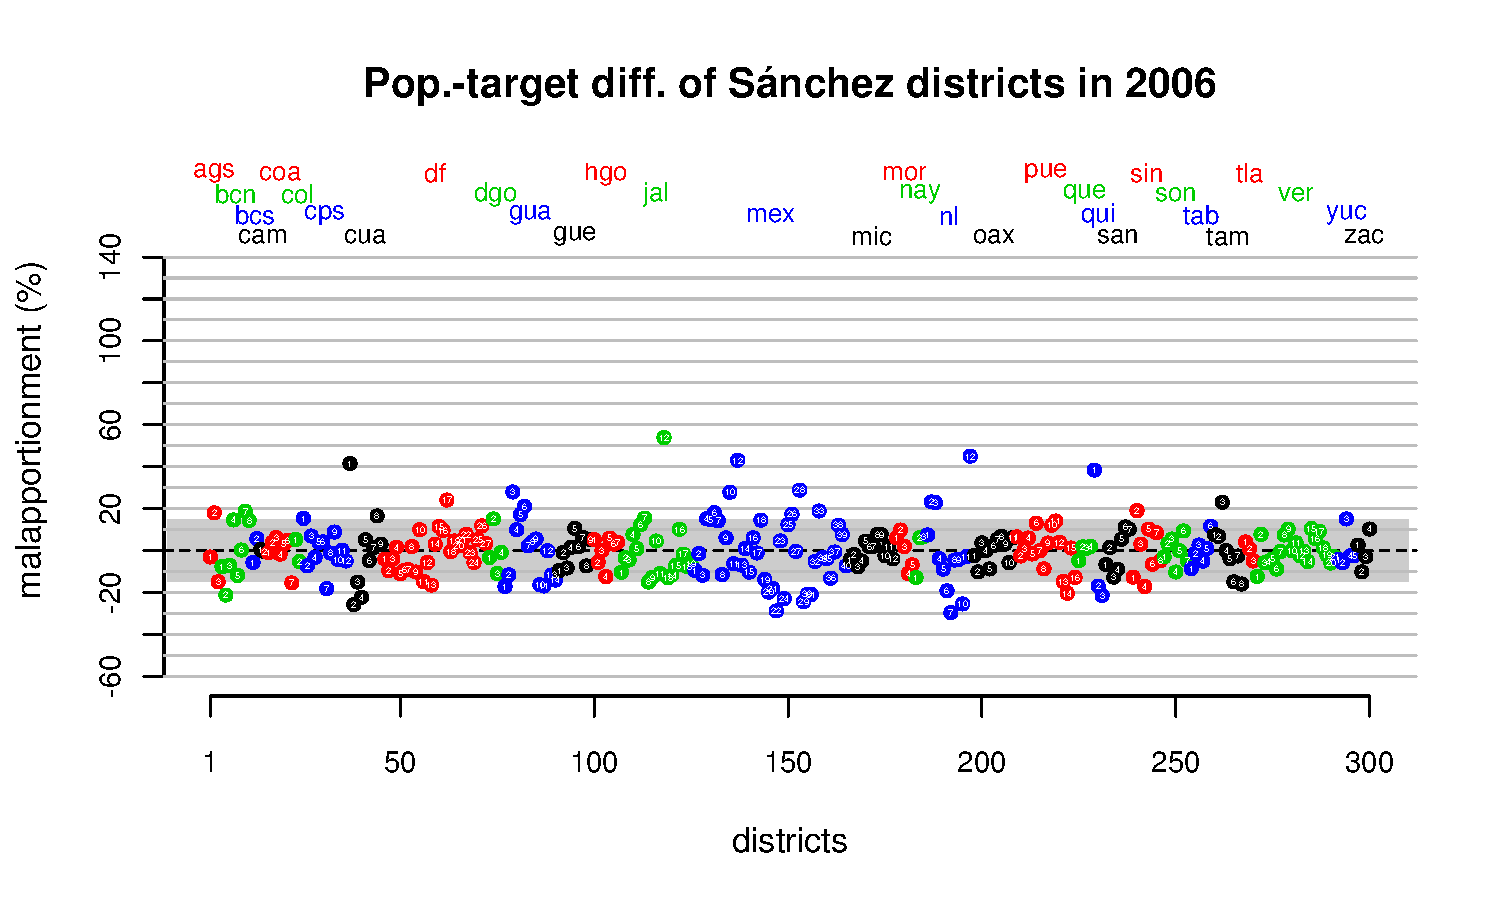
\includegraphics[width=.725\columnwidth]{malapp2006d0.pdf} \\
    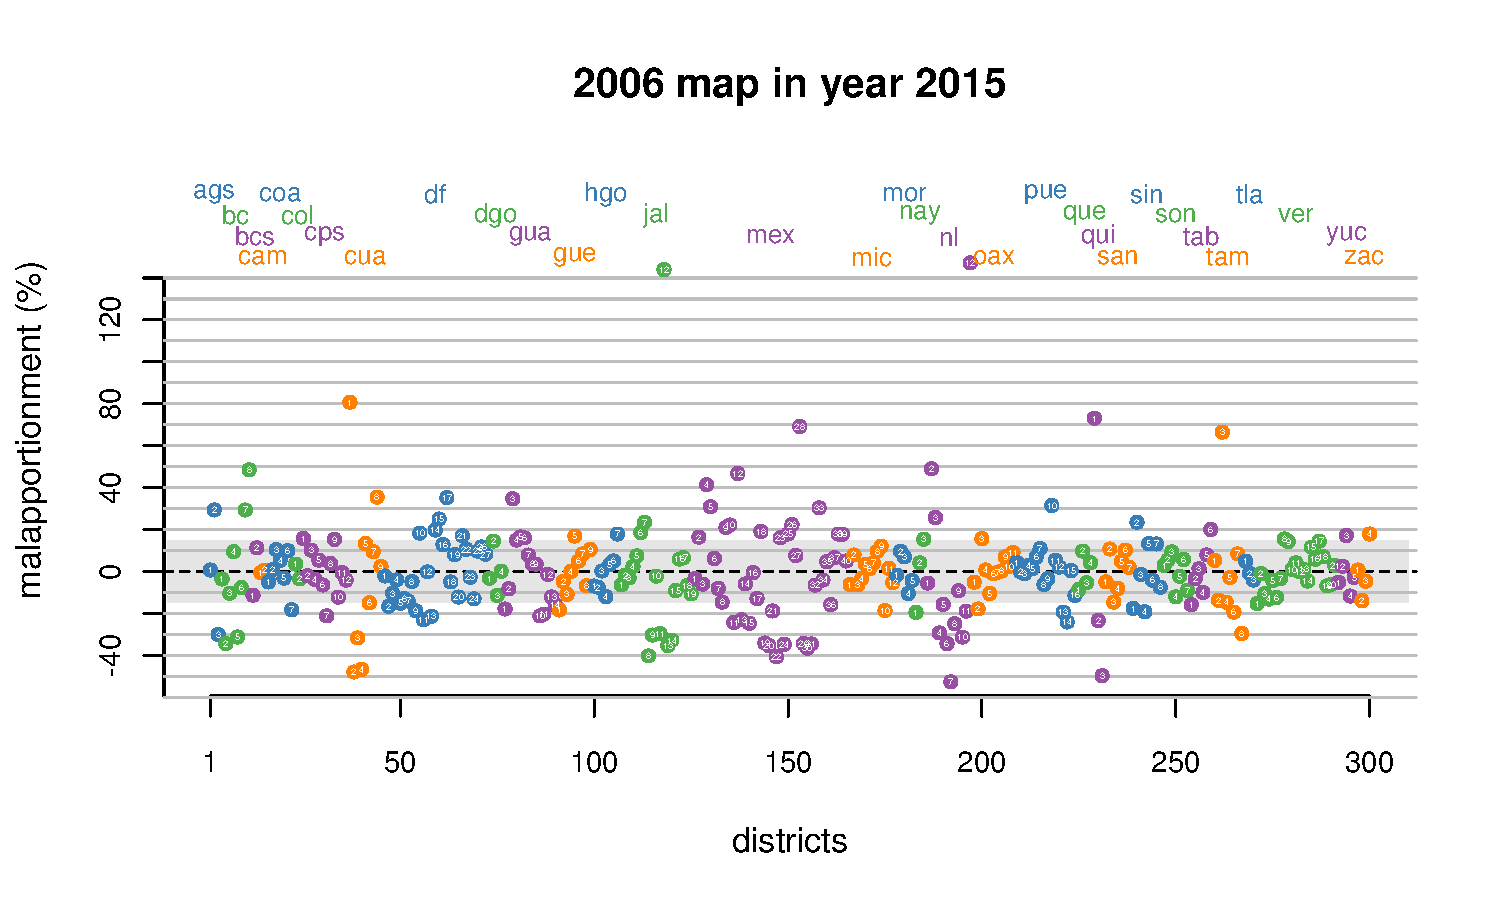
\includegraphics[width=.725\columnwidth]{malapp2015d0.pdf} \\
    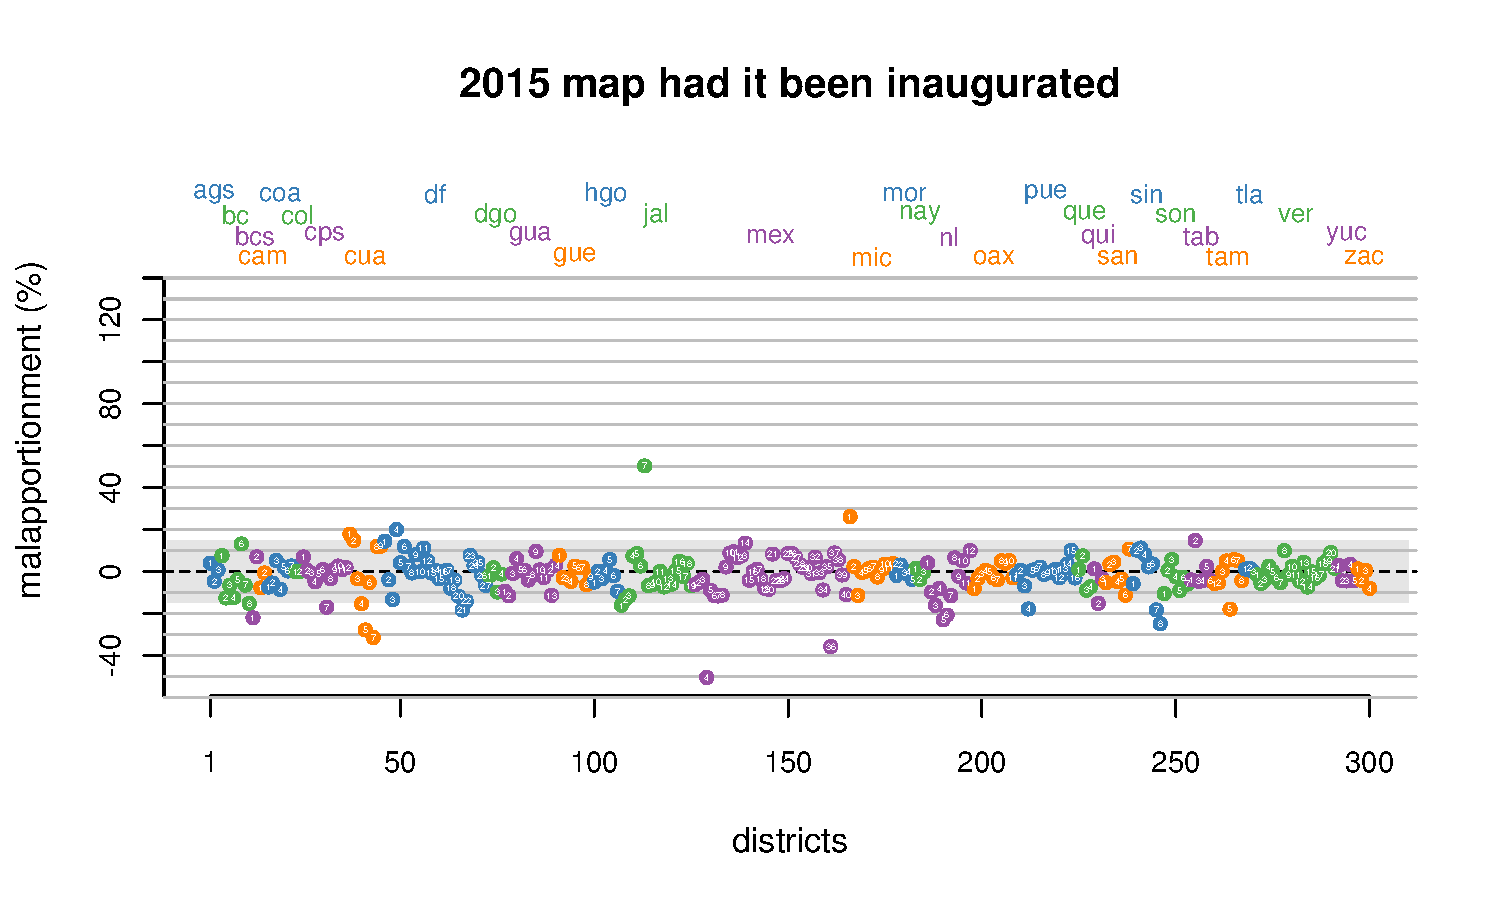
\includegraphics[width=.725\columnwidth]{malapp2015d3.pdf} \\
  \caption{Malapportionment through years and maps. The $y$-scale measures district population relative to ideal (mean state population). The grey band is IFE's range of tolerance for district population asymmetries.}\label{F:malapp}
\end{center}
\end{figure}

Small deviations around a state's mean district population are unavoidable. But what constitutes a small deviation remains a matter of opinion. Courts in the U.S. have struck down district maps bearing less than 1\% differences without proper justification \citep{tuckerApportionment.1985}. In sharp contrast, when redistricting towards 2006, IFE considered 10\% deviations perfectly normal. Towards 1997 and 2015, tolerance was greater, reaching 15\% above or below mean state district size. Within such spread, a district at the bottom end is worth one-third more in Congress than one at the top end. No party has ever challeged this in Court. 

Moreover, automated redistricting makes no attempt for maps to tend towards zero malapportionment, with only exceptional deviants within the range of tolerance. The preservation of municipal boundaries, for instance, is achieved by exploiting tolerated leeway. Figure \ref{F:malapp} shows how the tolerance band is uniformly occupied by districts even right after inception. It is notable that the new 2006 map had so many districts outside the range of tolerance. Difficulties to estimate population growth are partly responsible: the 2005 partial census was unavailable when the redistricting process began, and IFE had to guess. The mean linear extrapolation of 2006 state populations using the 1995--2000 rate of change is off by 2.8\% in absolute value and a standard deviation of 2\%. Variance cannot be smaller when dealing with sub-state units used to prepare districts, pushing about 80 new districts out of the broad $\pm 15$\% band.\footnote{Census data reported at the electoral section level are available since 2005 only. We could repeat this exercise at the municipal level to approximate IFE's mistakes better.} The requirement to keep municipalities with large indigenous population within the same district may also explain exceptions. Median absolute district malapportionent of the 2006 map upon inauguration was 6.5\%, the third quartile surpassing the ten point tolerance margin at 12.4\%. For the 2015 midterm election those descriptives will be 9.9 and 17.9\%, respectively. The 2015 map proposal did a better job upon inauguration, with median absolute district malapportionment of 4.2\% and third quartile at 8.1\%. 

\begin{tabular}{lrrrrr}
                 & \mc{5}{c}{Absolute malapportionment} \\
Map in year      & Min. & 1st quartile & median & 3rd quartile & max. \\ \hline
2006 map in 2006 & $<.01$ & 3.4 & 6.5 & 12.4 & 54.8 \\
2006 map in 2015 & .02 & 4.4 & 9.9 & 18.0 & 147.2 \\
2015 map in 2015 & .01 & 1.9 & 4.2 & 8.1 & 50.6 \\
\end{tabular}

Whether districts below and above fair representation behave differently merits closer inspection. Whether due to technical difficulties or discretion, malapportionment may be the source of meaningful distorsions in democratic representation.

\section{The 2006 map and the 2015 proposals}

*** Elements of Alejandro's discussion of redistricting process could fit well here. ***

A new map is a full description of district boundary changes. The common way to visualize a map is by drawing it. We look at maps differently, with focus not in the physical lines and line changes but in their political consequences. Putting the 2006 map and the 2015 final proposal drawings side to side reveals boundary shifts. But unless the drawing is more data rich, assessing even the relatively simple question of how similar districts were before and after redistricting visually is a challenge. 

\begin{table}
\begin{center}
  \begin{tabular}{lrrrrr}
  Similarity between                 &   min  &  25\%  & median &  75\% &  max \\ \hline
  first 2015 proposal and status quo & 0.128  & 0.419  & 0.584  & 0.755 &  1   \\
  final 2015 proposal and status quo & 0.125  & 0.437  & 0.643  & 0.805 &  1   \\
  first and final 2015 proposals     & 0.174  & 0.705  & 0.967  & 1     &  1   \\
  \end{tabular}
  \caption{District similarity before and after the failed 2015 redistricting}\label{T:simIndex}
\end{center}
\end{table}

But a similarity index \citep[][:15--7]{cox.katz.2002} offers ground for assessment. Measurement identifies the parent district or single largest contributor of population to every new district. The $s$imilarity index divides the population that $p$arent and $n$ew district share in $c$ommon by their joint population: $s = c / (p + n - c)$. The range is zero (district shares no population at all with parent) to one (districts are identical). Table \ref{T:simIndex} describes the change that the 2015 map would have brought in the 300 single member districts, comparing IFE's initial and final proposals with the 2006 map. Also compared are the final and initial 2015 proposals themselves. 

Six percent of districts entertained no change in boundaries whatsoever vis-\`a-vis the status quo (18 districts in the initial proposal, 19 in the final), and the proportion of districts with at least nine-tenths of the population in common doubles (40 in the initial, 44 in the final proposal). Inspecting which districts were a priori chosen for marginal or no change might reveal systematic distorsions of the automated redistricting algorithm. Party feedback left 39 percent of districts in IFE's first proposal intact, and 62 percent with up from nine-tenths of the population in common. Inspecting which districts the parties targeted for major amendment---presumably a partial restitution of a known and liked district from the status quo---should shed further light into the subject. Note how median district similarity with the 2006 map augmented from first to final proposal. So did the third quartile. Accepted counterproposals therefore restituted portions of status quo districts. This seems consistent with a view where parties protect strongholds that the algorythm may have split, but further analysis must be done. 

Noting that victory margins began widening in the mid-1960s, \citet{mayhew1974vanishingMg} saw gerrymandering as one possible explanation, incumbents influencing the preservation of safe districts. While the argument opened the heated incumbency advantage debate, the intuition may guide our inquiry. District volatility should capture a key element for analysis of map similarities. District $d$ volatility is $v_d = 1/2 \sqrt{ \sum_{p=1}^P \sum_{t=2}^3 (v_{d,p,t}- v_{d,p,t-1})^2 }$ with $p$ indexing the competing parties and $t=1,2,3$ for the 2006,  2009, and 2012 congressional elections respectively.\footnote{The measure of volatility proposed is inspired in measures of disroportionality, replacing the seats--votes difference with vote first differences. It is a squared version of a Loosemore-Hanby index \citep{loosemore.hanbyDisproportionality1971,gallagherDisproportionality1991}.} 

Mexican party strength is not proportional to the formidable entry barriers they enjoy and massive public subsidies they receive yearly \citep{magar.2007ref.2015}. Evidence of this is their inability to cultivate loyal voters. District volatility is remarkably high, as shown in Table \ref{T:volatMarginsd0}. The median district saw 25 percent of votes change party hands between 2006 and 2012 (not exactly how the index reads, but close enough). With so many volatile districts around, parties should have attempted to redress strongholds that automated redistricting split beyond recognition. How much were strongholds affected by the initial 2015 proposal? To what extent did party counterproposals redress them? This should be a promising line of inquiry. 

\begin{table}
\begin{center}
\begin{tabular}{lrrrrr}
                    &  min.   &  25\%   & median  & 75\%   & max \\ \hline
district volatility &  .08    & .19     & .25     & .31    & .52 \\
mean PAN margin     &  $-.49$ & $-.23$  & $-.10$  & .01    & .28 \\   
mean PRI margin     &  $-.43$ & $-.09$  & $-.01$  & .07    & .28 \\   
mean PRD margin     &  $-.51$ & $-.31$  & $-.21$  & $-.04$ & .39 \\
\end{tabular}
\caption{2006 map district volatility and party margins in three congressional elections}\label{T:volatMarginsd0}
\end{center}
\end{table}

[[One possibility is regressing new district similarity on mean 2006--12 parent district margin, low volatility, and their interaction.]]

[[Another route is the estimation of district elasticities---how vote swings in a district's sections respond to statetwide party swings. This could provide an alternative approach to explain the district similarity index. The appendix has prelimiary elasticity estimates and some discussion.]] 

\section{Winners and losers}

Party effects of redistricting should involve seat swaps, to which this section turns to. Counterfactual analysis answers how votes would have converted to seats in recent congressional elections had the 2015 redistricting proposal been used in stead of the status quo. M\'arquez (\href{http://bit.ly/1nk4kYs}{\url{http://bit.ly/1nk4kYs}}) did this using national-level data over two decades. I proceed with state-by-state breakdowns over much a shorter span (2006, 2009, and 2012), uncovering many seat changes that cancel out in the aggregate. Compared to the status quo, counterfactual districts would slightly benefit the PRI nationwide and, by alliance, the Green party, granting them 2 to 3 extra deputies; would slightly hurt the PAN, erasing 2 to 4 victories; and would, on average, leave the left unaffected. Analysis also reveals distributive effects in nearly half the states, which complicates the assessment of partisan effects of the redistricting proposal. Counterfactuals are prepared with IFE's first and final (third) 2015 redistricting proposals, offering perspective to appreciate whether and how parties influence expert electoral regulation in general \citep{estevez.magar.rosas.2008}, and district line drawing in particular \citep{rossiter.etal.1997,cox.katz.2002}. 

Column $S$ of Tables \ref{T:2006}, \ref{T:2009}, and \ref{T:2012} breaks down the federal deputy seats that parties won in the last three congressional elections by state (with actual districts). Columns $\Delta_1$ and $\Delta_3$ report seat changes had map proposals 1 and 3, respectively, been used instead. Changes are computed adding up section-level vote returns into districts. For the sake of readability, the tables do not distinguish seats that the PRI won with the Green party (PVEM) as coalition partner.\footnote{Nine states (two in 2009, seven in 2012) combining districts with joint PRI--Green candidate and districts where each fielded a candidate complicate counterfactual computation. Most counterfactual districts in such states blend sections with and without coalition votes, so a decision about their coalition status has to be made. I looked at whether or not coalition sections are the most numerous in the new district, classifying it accordingly. As a consequence, several seats won in status quo districts swap from the PRI to the coalition and vice versa in mixed states' counterfactuals---mostly in the State of Mexico 2009. Keeping such swaps in the count artificially inflates the redistributive effects of redistricting.} In 2009, PRI and partner competed against each other in 237 districts while fielding joint candidates in the remaining 63, and in 2012 they competed in 101 and shared candidate in 199. Coalition in 2006 was nationwide, like that of the PRD and two minor left parties in 2006 and 2009, removing complications. 

% pri coalition info:
% 2009
% 237 districts in 29 states with no coalition 
% 63 districts in 11 states with PRI-PVEM coalition
%  of which 46 districts in 9 states with mixed coalition status
% 2012
% 101 districts in 19 states with no coalition
% 199 districts in 13 srtates with PRI-PVEM coalition
%  of which XX in 7 states with mixed coalition status

\begin{table}
\begin{center}
 \begin{tabular}{rrrr|rrr|rrr}
      & \multicolumn{3}{c}{PAN} & \multicolumn{3}{c}{PRI coalition} & \multicolumn{3}{c}{PRD coalition} \\
state &$S$& $\Delta_1$ &  $\Delta_3$ & $S$& $\Delta_1$ &  $\Delta_3$ & $S$& $\Delta_1$ &  $\Delta_3$  \\ \hline
ags &   3 &     &     &      &      &      &      &      &        \\       
 bc &   8 &     &     &      &      &      &      &      &        \\       
bcs &     &     &     &      &      &      &    2 &      &        \\       
cam &     &     &     &    2 &      &      &      &      &        \\       \hdashline
coa &   5 & $-1$& $-1$&    2 &  $+1$&  $+1$&      &      &        \\       
col &   2 &     &     &      &      &      &      &      &        \\       
cps &     &     & $+1$&    7 &  $-1$&      &    5 &  $+2$&        \\       
cua &   4 & $+2$&     &    5 &  $-2$&      &      &      &        \\       \hdashline
 df &   2 &     &     &      &      &      &   25 &  $-3$&  $-3$  \\       
dgo &   1 & $+1$& $+1$&    3 &  $-1$&  $-1$&      &      &        \\       
gua &  14 & $+1$& $+1$&      &      &      &      &      &        \\       
gue &     &     &     &      &      &      &    9 &      &        \\       \hdashline
hgo &   1 &     &     &    4 &      &  $-1$&    2 &      &  $+1$  \\       
jal &  18 & $+1$& $+1$&    1 &      &      &      &      &        \\       
mex &  11 & $-1$&     &    6 &  $+1$&  $-1$&   23 &  $+1$&  $+2$  \\       
mic &   4 &     &     &      &      &      &    8 &      &        \\       \hdashline
mor &   2 &     & $-1$&    1 &  $-1$&      &    2 &  $+1$&  $+1$  \\       
nay &     &     &     &    2 &      &      &    1 &      &        \\       
 nl &   7 & $-1$& $-1$&    5 &  $+1$&  $+1$&      &      &        \\       
oax &     &     &     &    2 &      &      &    9 &  $-1$&  $-1$  \\       \hdashline
pue &  11 & $-1$& $-1$&    5 &  $-1$&      &      &  $+1$&        \\       
que &   4 & $+1$& $+1$&      &      &      &      &      &        \\       
qui &     &     &     &    2 &      &      &    1 &  $+1$&  $+1$  \\       
san &   7 &     &     &      &      &      &      &      &        \\       \hdashline
sin &   2 &     &     &    6 &  $-1$&  $-1$&      &      &        \\       
son &   5 &     &     &    2 &      &      &      &      &        \\       
tab &     &     &     &      &      &      &    6 &      &        \\       
tam &   5 & $+1$& $+1$&    3 &      &      &      &      &        \\       \hdashline
tla &   2 &     &     &      &      &      &    1 &      &        \\       
ver &  11 & $-3$& $-5$&    6 &  $+2$&  $+4$&    4 &      &        \\       
yuc &   4 & $-1$& $-1$&    1 &  $+1$&  $+1$&      &      &        \\       
zac &   1 &     &     &      &      &      &    3 &      &        \\ \hline 
tot & 134 & $-1$& $-4$&   65 &  $-1$&  $+3$&  101 &  $+2$&  $+1$  \\       
abs &     & $15$& $16$&      &  $13$&  $11$&      &  $10$&  $9$  \\       
\end{tabular}
\caption{Seats won by state and counterfactual differences in 2006. Columns $\Delta_1$ and $\Delta_3$ report change in $S$eats won with proposals 1 and 3 (discussed in text), respectively. Row tot reports column sum, row abs the sum of absolute column values.}\label{T:2006}
\end{center}
\end{table}


\begin{table}
\begin{center}
\begin{tabular}{rrrr|rrr|rrr|rrr}
      & \multicolumn{3}{c}{PAN} & \multicolumn{3}{c}{PRI$^*$} & \multicolumn{3}{c}{PRD} & \multicolumn{3}{c}{Other} \\
state &$S$& $\Delta_1$ &  $\Delta_3$ & $S$& $\Delta_1$ &  $\Delta_3$ & $S$& $\Delta_1$ &  $\Delta_3$ & $S$& $\Delta_1$ &  $\Delta_3$ \\ \hline
ags &   2 &     &     &   1 &     &     &     &     &      &    &    & \\       
 bc &   8 &     &     &     &     &     &     &     &      &    &    & \\       
bcs &     &     &     &     &     &     &   2 &     &      &    &    & \\       
cam &     &     &     &   2 &     &     &     &     &      &    &    & \\       \hdashline
coa &     &     &     &   7 &     &     &     &     &      &    &    & \\       
col &   1 &     &     &   1 &     &     &     &     &      &    &    & \\       
cps &   4 & $+1$& $-1$&   4 &     & $+3$&   4 &     & $-1$ &    &    & \\       
cua &   1 & $-1$& $-1$&   8 & $+1$& $+1$&     &     &      &    &    & \\       \hdashline
 df &   6 & $-1$& $-1$&   1 &     &     &  17 & $-2$& $-2$ & 3  &    & \\       
dgo &     &     &     &   4 &     &     &     &     &      &    &    & \\       
gua &  13 & $+1$& $+1$&   1 &     &     &     &     &      &    &    & \\       
gue &     &     &     &   8 &     &     &   1 &     &      &    &    & \\       \hdashline
hgo &     &     &     &   7 &     &     &     &     &      &    &    & \\       
jal &   9 & $+2$& $+3$&  10 & $-1$& $-2$&     &     &      &    &    & \\       
%mex &   2 &     &     &   8 & $-3$& $-2$&     &     &      &    &    & \\       
mex &   2 &     &     &  38 & $+1$& $+1$&     &     &      &    &    & \\       
mic &   4 & $+1$&     &     &     &     &   8 & $-1$&      &    &    & \\      \hdashline 
mor &     &     &     &   5 &     &     &     &     &      &    &    & \\       
nay &   1 &     &     &   1 &     &     &   1 &     &      &    &    & \\       
 nl &   5 & $-1$& $-1$&   7 & $+1$& $+1$&     &     &      &    &    & \\       
oax &     &     &     &  11 & $-1$& $-1$&     &     &      &    &    & \\       \hdashline
pue &     & $+2$& $+1$&  16 & $-3$& $-2$&     &     &      &    &    & \\       
que &   1 & $+1$&     &   3 &     & $+1$&     &     &      &    &    & \\       
qui &     &     &     &   3 & $+1$& $+1$&     &     &      &    &    & \\       
san &   5 &     &     &   2 &     &     &     &     &      &    &    & \\       \hdashline
sin &     & $+1$& $+1$&   8 & $-2$& $-2$&     &     &      &    &    & \\       
son &   2 &     &     &   5 &     &     &     &     &      &    &    & \\       
tab &     &     &     &   4 &     &     &   2 &     &      &    &    & \\       
tam &     &     &     &   8 & $+1$& $+1$&     &     &      &    &    & \\       \hdashline
tla &   3 &     &     &     &     &     &     &     &      &    &    & \\       
ver &   4 & $-2$& $-2$&  17 & $+1$& $+1$&     &     &      &    &    & \\       
yuc &     &     &     &   5 &     &     &     &     &      &    &    & \\       
zac &     &     &     &     &     &     &   4 &     &      &    &    & \\ \hline 
%tot &  71 & $+4$&     & 137 & $-6$& $-4$&  39 & $-3$& $-3$ & 3  &    & \\       
tot &  71 & $+4$&     & 187 & $-1$& $+3$&  39 & $-3$& $-3$ & 3  &    & \\       
abs &     & $14$& $12$&      &$13$& $17$&      & $3$&  $3$ &    &    & \\       
% \begin{tabular}{rrrr|rrr|rrr|rrr|rrr}
%       & \multicolumn{3}{c}{PAN} & \multicolumn{3}{c}{PRI} & \multicolumn{3}{c}{PRI coalition} & \multicolumn{3}{c}{PRD} & \multicolumn{3}{c}{Other} \\
% state &$S$& $\Delta_1$ &  $\Delta_3$ & $S$& $\Delta_1$ &  $\Delta_3$ & $S$& $\Delta_1$ &  $\Delta_3$ & $S$& $\Delta_1$ &  $\Delta_3$ & $S$& $\Delta_1$ &  $\Delta_3$ \\ \hline
% ags &   2 &     &     &   1 &     &     &      &      &      &     &     &      &    &    & \\       
%  bc &   8 &     &     &     &     &     &      &      &      &     &     &      &    &    & \\       
% bcs &     &     &     &     &     &     &      &      &      &   2 &     &      &    &    & \\       
% cam &     &     &     &   2 &     &     &      &      &      &     &     &      &    &    & \\       \hdashline
% coa &     &     &     &   7 &     &     &      &      &      &     &     &      &    &    & \\       
% col &   1 &     &     &   1 &     &     &      &      &      &     &     &      &    &    & \\       
% cps &   4 & $+1$& $-1$&     &     &     &    4 &      &  $+3$&   4 &     & $-1$ &    &    & \\       
% cua &   1 & $-1$& $-1$&   8 & $+1$& $+1$&      &      &      &     &     &      &    &    & \\       \hdashline
%  df &   6 & $-1$& $-1$&     &     &     &    1 &      &      &  17 & $-2$& $-2$ & 3  &    & \\       
% dgo &     &     &     &   4 &     &     &      &      &      &     &     &      &    &    & \\       
% gua &  13 & $+1$& $+1$&     &     &     &    1 &      &      &     &     &      &    &    & \\       
% gue &     &     &     &   6 &     &     &    2 &      &      &   1 &     &      &    &    & \\       \hdashline
% hgo &     &     &     &   6 &     &     &    1 &      &      &     &     &      &    &    & \\       
% jal &   9 & $+2$& $+3$&   7 & $-1$& $-2$&    3 &      &      &     &     &      &    &    & \\       
% %mex &   2 &     &     &   8 & $-3$& $-2$&   30 &  $+4$&  $+3$&     &     &      &    &    & \\       
% mex &   2 &     &     &     &     &     &$38^*$&  $+1$&  $+1$&     &     &      &    &    & \\       
% mic &   4 & $+1$&     &     &     &     &      &      &      &   8 & $-1$&      &    &    & \\      \hdashline 
% mor &     &     &     &   5 &     &     &      &      &      &     &     &      &    &    & \\       
% nay &   1 &     &     &   1 &     &     &      &      &      &   1 &     &      &    &    & \\       
%  nl &   5 & $-1$& $-1$&   7 & $+1$& $+1$&      &      &      &     &     &      &    &    & \\       
% oax &     &     &     &  11 & $-1$& $-1$&      &      &      &     &     &      &    &    & \\       \hdashline
% pue &     & $+2$& $+1$&  15 & $-3$& $-2$&    1 &      &      &     &     &      &    &    & \\       
% que &   1 & $+1$&     &   3 &     & $+1$&      &      &      &     &     &      &    &    & \\       
% qui &     &     &     &   1 &     &     &    2 &  $+1$&  $+1$&     &     &      &    &    & \\       
% san &   5 &     &     &   2 &     &     &      &      &      &     &     &      &    &    & \\       \hdashline
% sin &     & $+1$& $+1$&   8 & $-2$& $-2$&      &      &      &     &     &      &    &    & \\       
% son &   2 &     &     &   5 &     &     &      &      &      &     &     &      &    &    & \\       
% tab &     &     &     &   4 &     &     &      &      &      &   2 &     &      &    &    & \\       
% tam &     &     &     &   8 & $+1$& $+1$&      &      &      &     &     &      &    &    & \\       \hdashline
% tla &   3 &     &     &     &     &     &      &      &      &     &     &      &    &    & \\       
% ver &   4 & $-2$& $-2$&  17 & $+1$& $+1$&      &      &      &     &     &      &    &    & \\       
% yuc &     &     &     &     &     &     &    5 &      &      &     &     &      &    &    & \\       
% zac &     &     &     &     &     &     &      &      &      &   4 &     &      &    &    & \\ \hline 
% %tot &  71 & $+4$&     & 137 & $-6$& $-4$&   50 &  $+5$&  $+7$&  39 & $-3$& $-3$ & 3  &    & \\       
% tot &  71 & $+4$&     & 129 & $-3$& $-2$&$58^*$&  $+2$&  $+5$&  39 & $-3$& $-3$ & 3  &    & \\       
\end{tabular}
\caption{Seats won by state and counterfactual differences in 2009. See Table \ref{T:2006} for column and row label meanings. $^*$Includes 50 seats that the PRI won in coalition in 63 districts from 10 states.}\label{T:2009}
% \caption{Seats won by state and counterfactual differences in 2009. See Table \ref{T:2006} for column label meanings. $^*$Includes 8 seats the PRI won solo, see text for details.}\label{T:2009} 
\end{center}
\end{table}


\begin{table}
\begin{center}
\begin{tabular}{rrrr|rrr|rrr|rrr}
      & \multicolumn{3}{c}{PAN} & \multicolumn{3}{c}{PRI$^*$} & \multicolumn{3}{c}{PRD coalition} & \multicolumn{3}{c}{Other} \\
state &$S$& $\Delta_1$ &  $\Delta_3$ & $S$& $\Delta_1$ &  $\Delta_3$ & $S$& $\Delta_1$ &  $\Delta_3$ & $S$& $\Delta_1$ &  $\Delta_3$ \\ \hline
ags &   2 & $-1$& $-1$&   1 & $+1$& $+1$&      &      &       &    &    & \\       
 bc &   1 &     &     &   7 &     &     &      &      &       &    &    & \\       
bcs &   2 &     &     &     &     &     &      &      &       &    &    & \\       
cam &     &     &     &   2 &     &     &      &      &       &    &    & \\       \hdashline
coa &   3 &     &     &   4 &     &     &      &      &       &    &    & \\       
col &     &     &     &   2 &     &     &      &      &       &    &    & \\       
cps &     &     &     &   9 & $+1$& $+2$&      &      &       & 3  &    & $-1$ \\       
cua &   1 & $-1$&     &   8 & $+1$&     &      &      &       &    &    & \\       \hdashline
 df &   1 &     &     &     &     &     &   26 &  $-3$&  $-3$ &    &    & \\       
dgo &     &     &     &   4 &     &     &      &      &       &    &    & \\       
gua &   7 & $+2$& $+2$&   7 & $-1$& $-1$&      &      &       &    &    & \\       
gue &     &     &     &     &     &     &    9 &      &       &    &    & \\       \hdashline
hgo &     &     &     &   7 &     &     &      &      &       &    &    & \\       
jal &   1 &     &     &  18 &     &     &      &  $+1$&  $+1$ &    &    & \\       
mex &   1 & $-1$& $-1$&  31 & $+3$& $+2$&    8 &  $-1$&       &    &    & \\       
mic &     &     &     &   8 & $+1$&     &    4 &  $-1$&       &    &    & \\       \hdashline
mor &     &     &     &   1 &     &     &    4 &      &       &    &    & \\       
nay &     &     &     &   3 &     &     &      &      &       &    &    & \\       
 nl &   6 & $-2$& $-2$&   6 & $+2$& $+2$&      &      &       &    &    & \\       
oax &     &     &     &   1 & $-1$& $-1$&   10 &      &       &    &    & \\       \hdashline
pue &   4 & $-1$&     &  12 & $-1$& $-2$&      &  $+1$&  $+1$ &    &    & \\       
que &   2 & $+1$& $+1$&   2 &     &     &      &      &       &    &    & \\       
qui &     &     &     &   2 &     &     &    1 &  $+1$&  $+1$ &    &    & \\       
san &   2 & $+1$&     &   5 & $-1$&     &      &      &       &    &    & \\       \hdashline
sin &   2 &     &     &   6 & $-1$& $-1$&      &      &       &    &    & \\       
son &   5 &     &     &   2 &     &     &      &      &       &    &    & \\       
tab &     &     &     &     &     &     &    6 &      &       &    &    & \\       
tam &   6 & $-1$& $-1$&   2 & $+2$& $+2$&      &      &       &    &    & \\       \hdashline
tla &     &     &     &   1 &     &     &    2 &      &       &    &    & \\       
ver &   5 & $+1$&     &  15 & $-2$& $-1$&    1 &      &       &    &    & \\       
yuc &   1 &     &     &   4 &     &     &      &      &       &    &    & \\       
zac &     &     &     &   4 &     &     &      &      &       &    &    & \\ \hline
tot &  52 & $-2$& $-2$& 174 & $+4$& $+3$&   71 &  $-2$&       & 3  &    & $-1$ \\       
abs &     & $12$& $8$ &      &$18$& $15$&      &  $8$ &  $6$  &    &    & $2$  \\       
% \begin{tabular}{rrrr|rrr|rrr|rrr|rrr}
%       & \multicolumn{3}{c}{PAN} & \multicolumn{3}{c}{PRI} & \multicolumn{3}{c}{PRI coalition} & \multicolumn{3}{c}{PRD coalition} & \multicolumn{3}{c}{Other} \\
% state &$S$& $\Delta_1$ &  $\Delta_3$ & $S$& $\Delta_1$ &  $\Delta_3$ & $S$& $\Delta_1$ &  $\Delta_3$ & $S$& $\Delta_1$ &  $\Delta_3$ & $S$& $\Delta_1$ &  $\Delta_3$ \\ \hline
% ags &   2 & $-1$& $-1$&   1 & $+1$& $+1$&      &      &      &      &      &       &    &    & \\       
%  bc &   1 &     &     &     &     &     &    7 &      &      &      &      &       &    &    & \\       
% bcs &   2 &     &     &     &     &     &      &      &      &      &      &       &    &    & \\       
% cam &     &     &     &   1 &     &     &    1 &      &      &      &      &       &    &    & \\       \hdashline
% coa &   3 &     &     &   4 &     &     &      &      &      &      &      &       &    &    & \\       
% col &     &     &     &     &     &     &    2 &      &      &      &      &       &    &    & \\       
% cps &     &     &     &     &     & $+1$&    9 &  $+1$&  $+1$&      &      &       & 3  &    & $-1$ \\       
% cua &   1 & $-1$&     &   8 & $+1$&     &      &      &      &      &      &       &    &    & \\       \hdashline
%  df &   1 &     &     &     &     &     &      &      &      &   26 &  $-3$&  $-3$ &    &    & \\       
% dgo &     &     &     &   4 &     &     &      &      &      &      &      &       &    &    & \\       
% gua &   7 & $+2$& $+2$&     &     &     &    7 &  $-1$&  $-1$&      &      &       &    &    & \\       
% gue &     &     &     &     &     &     &      &      &      &    9 &      &       &    &    & \\       \hdashline
% hgo &     &     &     &   7 &     &     &      &      &      &      &      &       &    &    & \\       
% jal &   1 &     &     &     &     &     &   18 &      &      &      &  $+1$&  $+1$ &    &    & \\       
% mex &   1 & $-1$& $-1$&     &     &     &   31 &  $+3$&  $+2$&    8 &  $-1$&       &    &    & \\       
% mic &     &     &     &   6 & $+1$&     &    2 &      &      &    4 &  $-1$&       &    &    & \\       \hdashline
% mor &     &     &     &     &     &     &    1 &      &      &    4 &      &       &    &    & \\       
% nay &     &     &     &   3 &     &     &      &      &      &      &      &       &    &    & \\       
%  nl &   6 & $-2$& $-2$&     &     &     &    6 &  $+2$&  $+2$&      &      &       &    &    & \\       
% oax &     &     &     &   1 & $-1$& $-1$&      &      &      &   10 &      &       &    &    & \\       \hdashline
% pue &   4 & $-1$&     &   1 &     &     &   11 &  $-1$&  $-2$&      &  $+1$&  $+1$ &    &    & \\       
% que &   2 & $+1$& $+1$&   1 &     &     &    1 &      &      &      &      &       &    &    & \\       
% qui &     &     &     &     &     &     &    2 &      &      &    1 &  $+1$&  $+1$ &    &    & \\       
% san &   2 & $+1$&     &   4 &     &     &    1 &  $-1$&      &      &      &       &    &    & \\       \hdashline
% sin &   2 &     &     &   6 & $-1$& $-1$&      &      &      &      &      &       &    &    & \\       
% son &   5 &     &     &   2 &     &     &      &      &      &      &      &       &    &    & \\       
% tab &     &     &     &     &     &     &      &      &      &    6 &      &       &    &    & \\       
% tam &   6 & $-1$& $-1$&   2 & $+2$& $+2$&      &      &      &      &      &       &    &    & \\       \hdashline
% tla &     &     &     &   1 &     &     &      &      &      &    2 &      &       &    &    & \\       
% ver &   5 & $+1$&     &     &     &     &   15 &  $-2$&  $-1$&    1 &      &       &    &    & \\       
% yuc &   1 &     &     &     &     &     &    4 &      &      &      &      &       &    &    & \\       
% zac &     &     &     &     &     &     &    4 &      &      &      &      &       &    &    & \\ \hline
% tot &  52 & $-2$& $-2$&  52 & $+3$& $+2$&  122 &  $+1$&  $+1$&   71 &  $-2$&       & 3  &    & $-1$ \\       
\end{tabular}
\caption{Seats won by state and counterfactual differences in 2012. See Table \ref{T:2006} for column and row label meanings. $^*$Includes 122 seats that the PRI won in coalition in 199 districts from 17 states.}\label{T:2012}
\end{center}
\end{table}

Seen from the national level (bottom line in each table), distributive effects are quite small. The largest drop observed is 4 seats subtracted from PAN in 2006 by the third proposal ($\Delta_3$), the largest hikes 4 extra seats for PAN in 2006 and PRI in 2009 by the first proposal ($\Delta_1$). Mean changes in the period are milder: proposal 1 returns $+\frac{1}{3}$ seat for PAN on average, $+\frac{2}{3}$ for PRI, and $-1$ for PRD; proposal 3 returns $-2$ for PAN, $+3$ for PRI, and $-\frac{2}{3}$ for the left. Adjustments made from first to final proposal are interesting. Party feedback turned the PRI from loser of one seat to winner of three in both 2006 and 2009, a net change of $\bar{\Delta_3} - \bar{\Delta_1} = 4$. Party feedback hurt the PAN almost simmetrically those years, with net changes between $-3$ and $-4$. The puzzle is that PAN had the most counterproposals accepted (see Table \ref{T:counterprops}), which coud be explained by a priority to preserve margins in strongholds and not just victories. Our analysis could presumably show this. 

Changes nationally do not reach one percent of the full chamber. Yet putting them in contrast with recent events in the electoral arena somewhat increases their relevance. Three deputies more is one-third what the PRI--Green coalition lacks to achieve majority status in the 62nd Legislature (2012--15). And it would have sufficed to win three seats from the PRI in 2000 for the PAN to enjoy the plurality in the chamber in the 58th Legislature (2000--03). In a world of volatile voters and tight margins, characteristic of present-day Mexico, a small difference can have larger consequences. 

National aggregates hide substantive redistricting effects at the state level. In 2006, the year most sensible to redistricting, seat distributions change in 18 states (of 32) with the proposals, but positives and negatives tend to cancel out in the national sum. The sum of absolute state changes---the bottom row of each table---reveals how many seat swaps (both for and against) a party experiences with redistricting. That year, the PAN, PRI and PRD would have had 16, 11, and 9 such swaps with the third redistricting proposal, respectively. These figures are between 4 and 9 times larger than national changes. In fact, the PAN's 2009 and PRD's 2012 nil nationwide changes are the sum of, respectively, 12 and 6 statewide absolute swaps that fully cancel one another. Some states by themselves involve larger distributive effects than the party's national total, as was the case of 2009 in Veracruz (PAN would get 5 seats less, PRI 4 more) and Jalisco (PAN would get 3 more seats). 

Eleven seats would swap state party hands in 2006 with the adoption of the third proposal, four in the state of Veracruz only. This count excludes seat changes due to reapportionment---seats that one state party wins or loses with no impact on another's seats\footnote{Based on the last decade's population shifts, seven states are bound to get an extra federal seat (Chiapas, Guanajuato, Jalisco, M\'exico, Qur\'etaro, Quintana Roo, and Tamaulipas), four to lose one (Oaxaca, Puebla, Sinaloa, Veracruz) and the Federal District to lose 3.}---yet is nearly three times larger than national swaps. The ratio of state party seat swaps to national party seat swaps in 2009 and 2012 (ten and eight, respectively) remains about 3. 

All said, inspection of counterfactuals through the lens of recent electoral history suggests that the adoption of the redistricting proposal would have helped the PRI. That party managed to redress district lines in the party--IFE negotiations to avoid likely seat losses and get likely bonus seats instead. The regulator's decision to celebrate the 2015 midterm congressional election with outdated districts appears to postpone pain for the PAN and the left one election cycle. 


\section{Party bias and responsiveness}

This section estimates district responsivity and party bias---two effects of scholarly interest, discussed below. M\'arquez (\href{http://bit.ly/1jgsQXE}{\url{http://bit.ly/1jgsQXE}}) has also approached this with national aggregates, uncovering a degree of responsivity characteristic of Westminster systems and party bias against the PAN under the status quo. By proceeding with state aggregates, much higher responsivity (owing to fewer districts, 9 by state on average) is uncovered, but no apparent party bias in neither the 2006 map nor 2015 proposals. 

\subsection{Systematic bias}

\begin{figure}
\begin{center}
    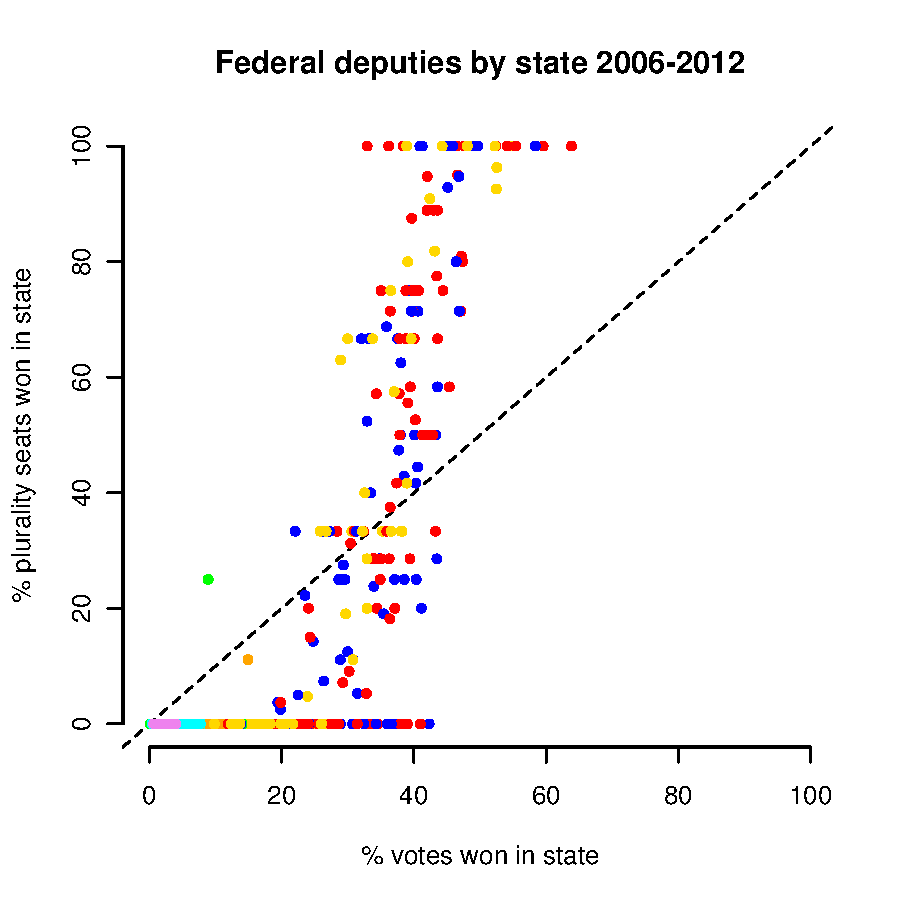
\includegraphics[width=.6\columnwidth]{resXedo20062012.pdf} 
\caption{Seats and votes in the states. Each point is a party-state-year, blue for PAN, red for PRI, gold for PRD, other colors for minor parties.}\label{F:seatsVotes}
\end{center}
\end{figure}

Consider now the relation between party votes and seats portrayed in Figure \ref{F:seatsVotes}. As before, the plot considers plurality seats only and state aggregates. Each point reports the vote share that a party won in a state's federal deputy elections (x-axis) and the share of the state's congressional seats it received (y-axis). Colors distinguish the parties: PAN is blue, PRI is red, PRD is gold, Green is green, among others. For instance, the green dot floating to the left of the cloud is the Green party in Chiapas 2012, where it won 3 of 12 districts. The chart shows that 9 percent of the state's vote awarded the party 25 percent of the seats, an outstanding achievement for any party. The cloud manifests a steep upwards slope characteristic of first-past-the.post systems \citep{taagepera.CubeLaw.1973}.\footnote{Adding the excluded PR seats would level the slope considerably. Doing this would be easy with national aggregates. It is not evident how to carry it with state aggregates, since PR seats are awarded in five second-tier districts joining together several states each.} Points below the diagonal indicate under-representation, those above over-representation. There are notable differences among major parties: the PRI achieved over-representation in three-fifths of election-states between 2006 and 2012, the PAN in two-fifths, and the PRD in one-fourth only. 

With such setting, the possibility that districts are granting undue advantage to the PRI merits closer inspection. A priori, reasons to suspect IFE of cooking districts to favor one party or another are lacking. Major parties, after all, permanently influence the election regulator, ambition counteracting ambition \citep{estevez.magar.rosas.2008}. But that those who draw the district lines can distort a fundamental link of the democratic process is well established in the literature \citep{altman.mcdonald2011bard,cox.katz.2002,engstrom2006redisttrictApsr,rossiter.etal.1997,king.1990elRespBiasMultiparty,balinskiYoung2001FairRep,otero.2003}. Has the insidious gerrymandering reared its ugly head in Mexico? This section estimates majority and party effects in the proposed districts and the status quo. Majority effects are huge, partisan effects negligible. 

\subsection{Two classes of distorsion}

Undue advantage is known, in the specialized literature, as partisan bias, and is one goal that strategic redistricters pursue. It is not, however, alone: scholarship highlights district responsiveness, also know as majoritarian bias, as another goal. These ought to be distinguished \citep[this paragraph draws heavily on][, ch.\ 3]{cox.katz.2002}. Partisan bias helps the beneficiary buy seats with fewer votes than others. Because seat distribution is a constant sum game, bias in favor of someone always implies bias against someone else. One way of introducing party bias in district lines is with the conventional redistricting strategy known as packing: group your adversary's voters in few districts, wasting votes to win unnecessarily safe seats, raising the price of victory. Responsiveness, on the other hand, is the feature granting a seat bonus to large parties. Maximal responsiveness occurs within each single-member district in isolation: the winner takes all, the rest nothing. The same could be achieved in a whole state by drawing lines so that every district is representative of the state's electorate (Cox and Katz's microcosm strategy). The party with most votes wins every seat, maximizing the vote responsiveness of the proposal. 

Formalizing party bias and responsiveness opens the way towards estimation of these district characteristics. The two-party case is simpler and extends to multiparty systems \citep{taagepera.CubeLaw.1973,tufte1973seatsVotes,king.browning1987biasRespUS}. It is a generalization of the cube law stipulating that 

\begin{equation}
 \frac{s}{1-s} = e^\lambda *  \left(\frac{v}{1-v}\right)^\rho \iff
 \texttt{logit}(s) = \lambda + \rho *  \texttt{logit}(v)
\end{equation}\label{E:cubeLaw}

\noindent where $s$ is the seat share that party 1 won with vote share $v$; $\lambda$ is party 1's bias relative to party 2 (positive values favor party 1, negative values favor party 2); and $\rho$ is the districts' responsiveness. With $\lambda=0$ a system with no party bias ensues. Figure \ref{F:lambdaRhoEx} shows how the parameters affect the vote-to-seats conversion. 

\begin{figure}
\begin{center}
    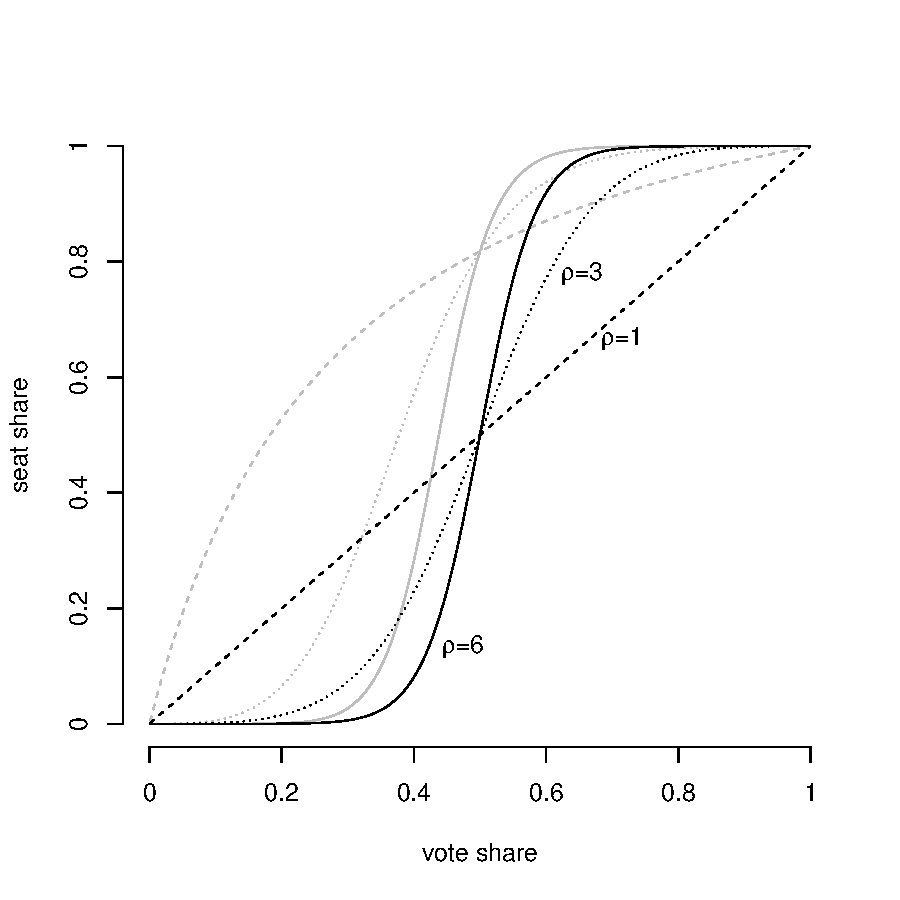
\includegraphics[width=.55\columnwidth]{rhoExample.pdf} 
\caption{Illustration of estimated parameters. Party bias is set to $\lambda=0$ in non-grey lines. Grey lines replicate the colored ones with $\lambda=+1.5$.}\label{F:lambdaRhoEx}
\end{center}
\end{figure}

Non-grey lines lack party bias to illustrate variable responsiveness. A system with $\rho=1$ is perfectly proportional representation, the ideal type against which the evaluation of real districts are often contrasted. It appears as the dotted green diagonal: every party winning $x$\% of the vote gets, precisely, $x$\% of seats. $\rho=3$ characterizes the classic cube law, the red curve over-representing the winner (points above the diagonal). Here a party with 55\% of the vote earns two-thirds of the seats, but with 33\% it earns only one-tenth of the seats. As responsivity grows, the curve gets steeper, until barely crossing the majority threshold suffices to win all the available seats. 

Grey lines replicate the values of $\rho$ just discussed but with $\lambda = 1.5$ added. Bias in favor of the party produces a leftward pull of lines. In other words, a bias-favored party requires less effort to reach the threshold for large-party over-representation. (The grey dotted line demonstrates how, due to logit links in Equation 1, party bias also reshapes the function's trace.)

A multiparty and estimable version of equation 1 \citep{king.1990elRespBiasMultiparty} establishes that party $j$'s ($j=1,2,\ldots,J$) expected seat share is 
\begin{equation}
 E(s_j) = \frac{e^{\lambda_j} * v_j^\rho}{\sum_{m=1}^{J} e^{\lambda_m} * v_m^\rho}
\end{equation}

\noindent with data and parameters indexed to identify the parties. \citep[Another, with application to Argentine federalism, is][.]{calvo.micozzi.govReform.2005} Setting $\lambda_2 = 0$, as done below, forces the remainder $\lambda_{j \neq 2}$ to express party bias with relation to the PRI's ($j=2$ for this party in the dataset). This is convenient to test the presumption of PRI-favoring bias:. if present, $\hat{\lambda}_{j \neq 2}<0$ would result.

A common estimation strategy relies on a time-series of national aggregates (this is what M\'arquez did for eight elections 1991--2012, uncovering substantive anti-PAN bias and high responsiveness). The estimation strategy here, as before, is with state-level data. One disadvantage of the approach is that states have few districts (9.4 on average), and this will amplify the system's responsiveness \citep{taagepera.CubeLaw.1973}. The advantages are many. The approach mutiplies observations. This is evident in Figure \ref{F:seatsVotes}, with many points despite reporting three elections only. It holds the actual district structure constant---rediustricting in 1997 and 2006 invalidates district comparability before and after. And it takes advantage in the variation of state party systems (this draft fails to take full advantage of this variance, but this could be exploited further). 

\begin{figure}
\begin{center}
  \begin{tabular}{cc}
    (a) & (b) \\
    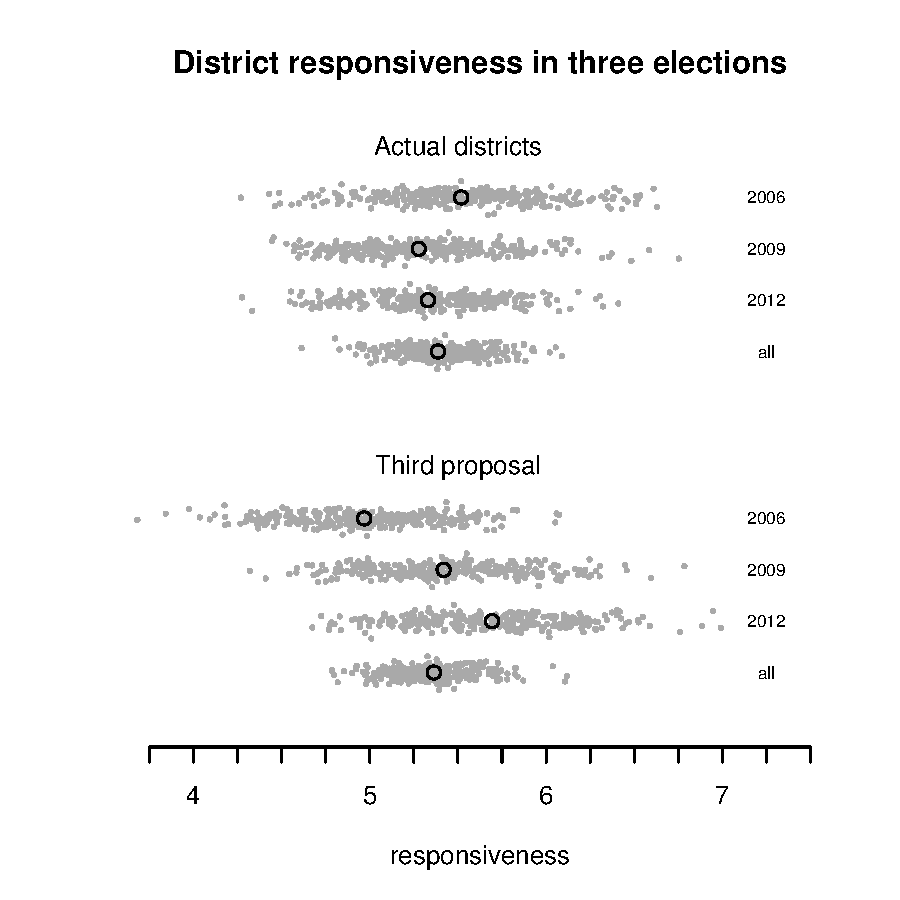
\includegraphics[width=.45\columnwidth]{resp200612s0s3.pdf} &
    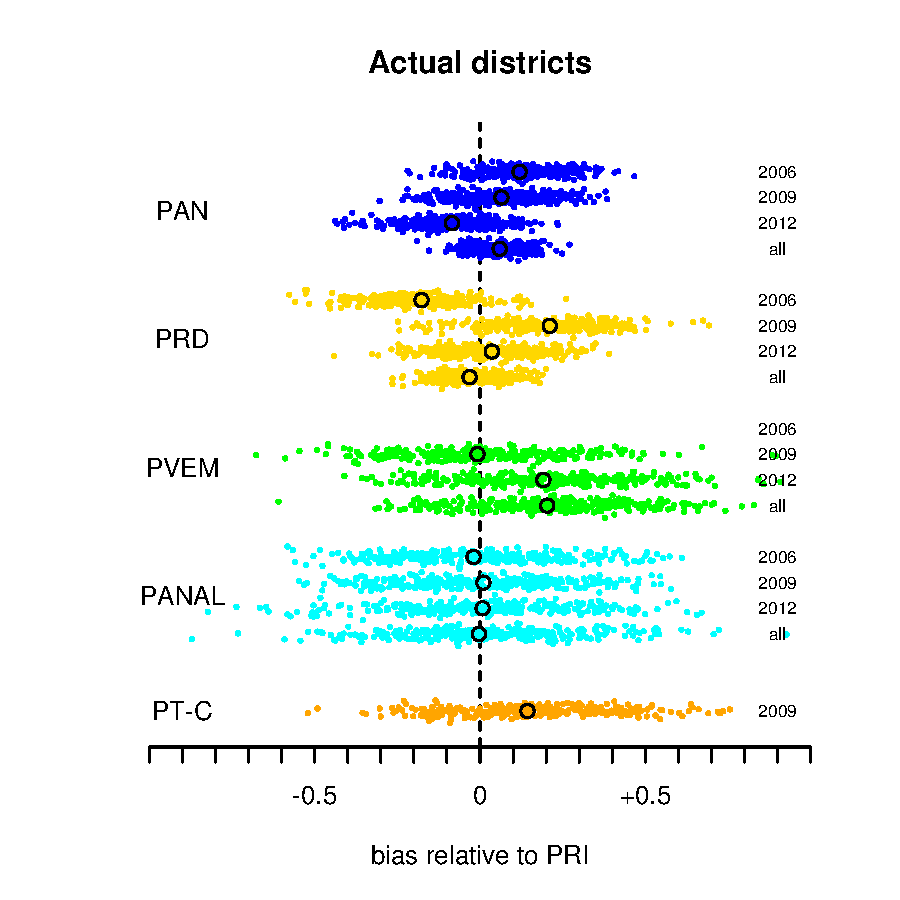
\includegraphics[width=.45\columnwidth]{bias200612s0.pdf} \\
    (c) & (d) \\
    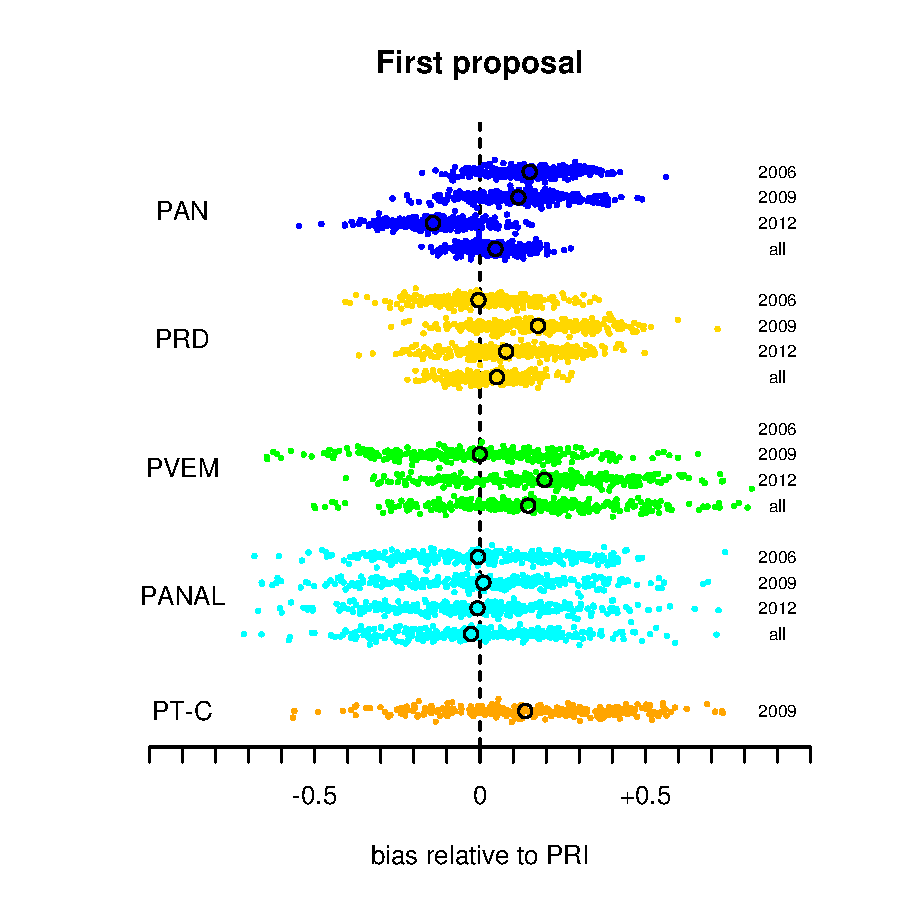
\includegraphics[width=.45\columnwidth]{bias200612s1.pdf} &
    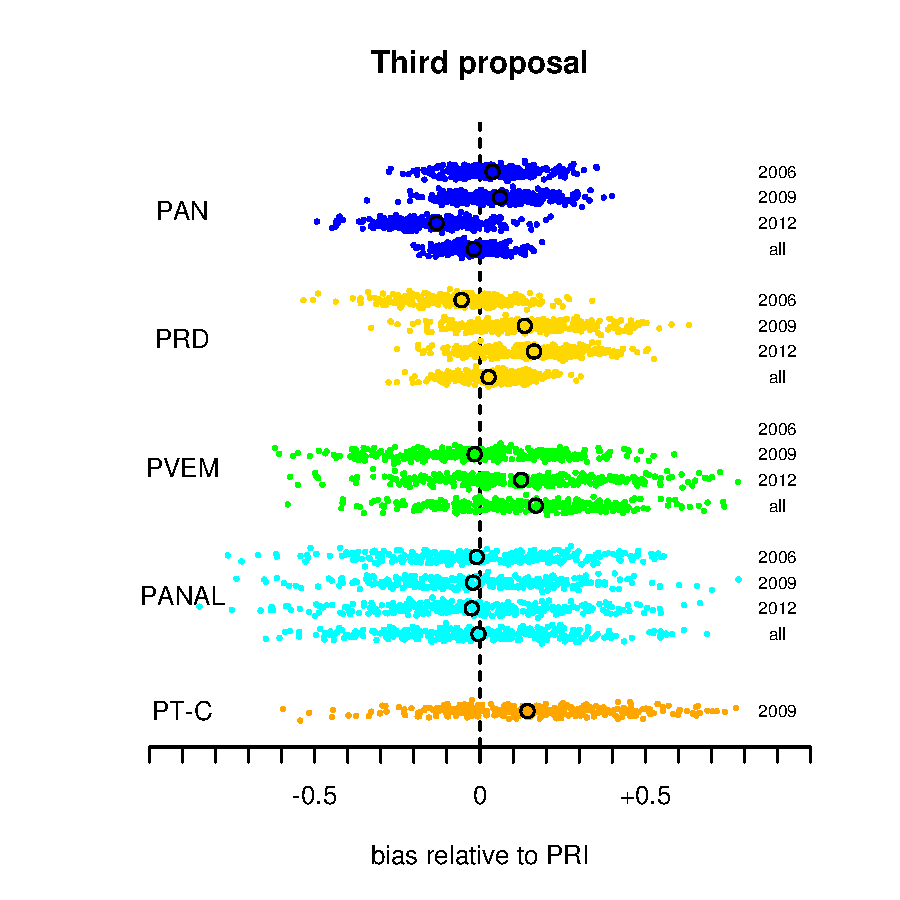
\includegraphics[width=.45\columnwidth]{bias200612s3.pdf} 
  \end{tabular}
  \caption{Redistricting, responsiveness, and party bias. Plots report the posterior sample of model's parameters $\lambda_j$ for four parties and $\rho$, and the median value (black circles).}\label{F:posterior_s0s1s3}
\end{center}
\end{figure}


The  method of estimation is MCMC \citep{jackman.2000}.\footnote{Three chains were iterated 10 thousand times, taking every fiftieth observation of the last 5 thousand to sample the posterior distribution. Convergence was gauged visually with traceplots of the separate chains for each of the model's parameters. Estimation performed with JAGS \citep{jags.cite}, implemented from R \citep{r.cite} using package R2jags \citep{r.r2jags}. Data and code to replicate the analysis can be found at HTTP.} As expected, district responsiveness is extremely high, between 5 and 6 depending on the year selected (the steepest line in illustrative Figure \ref{F:lambdaRhoEx} has $\lambda=6$). Figure \ref{F:posterior_s0s1s3}.a reports point estimates (the black circles are the median of the posterior sample of the responsiveness parameter) for each year separately, all years pooled together, and comparing actual districts to the first and third redistricting proposals. Estimate precision is assessed with the cloud of grey points (technically, it is the full sample of posterior $\rho$s). The redistricting proposal makes little change to district responsiveness, it just makes it slightly more volatile from one election to next. Owing to few districts per state, the estimated responsiveness at the state level ($\hat{\rho} \approx 5.5$) is twice M\'arquez's nationwide ($\hat{\rho} = 2.6$). All three parties experience situations of large party bonus and small party penalty that, to a good extent, cancel each other in the national statistic.

Regarding party bias, signals that are not weak all tend to be accompanied by a good deal of noise, with few exceptions. At the national level, and over a longer haul, M\'arquez discovers bias in favor of the PRI, but mostly in favor of the PRD, and against the PAN, that seems not the product of chance alone. Analysis at the state-level reveals no such biases. As said, Figures \ref{F:posterior_s0s1s3}.b--d express bias relative to the PRI. Although PAN experienced weak signal in its favor in the whole 2006--12 period, a fair density of the blue cloud is, in fact, negative. PRD vs.\ PRI bias is clearly centered at zero in the full period. The left did experience significant bias in isolated years: against in 2006, in favor in 2009. Perhaps voters who strategically abandoned the hopeless PRI presidential candidate in 2006 to vote for L\'opez Obrador did not also endorse the PRD's congressional candidates. No other year for no other party reveals any bias unaccompanied by much noise.

% \section{Malapportionment and margin}

% \begin{figure}
% \begin{center}
%   \begin{tabular}{cc}
%     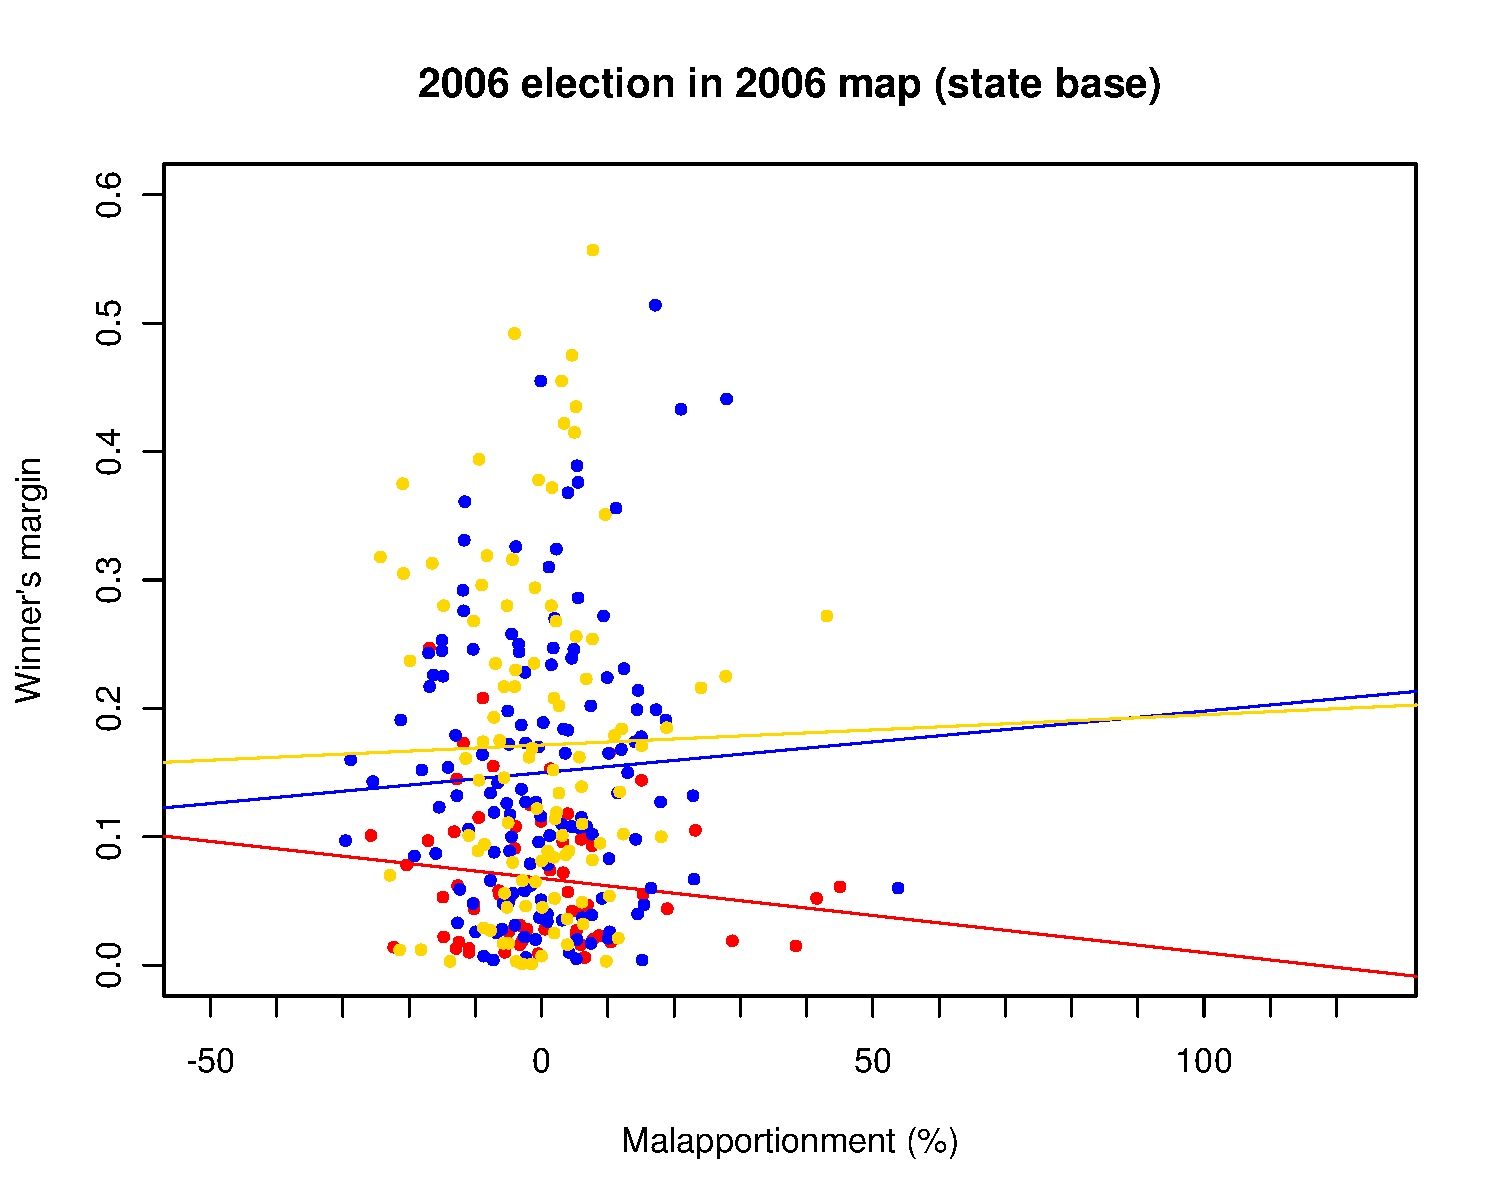
\includegraphics[width=.4\columnwidth]{malmg2006d0sta.pdf} & 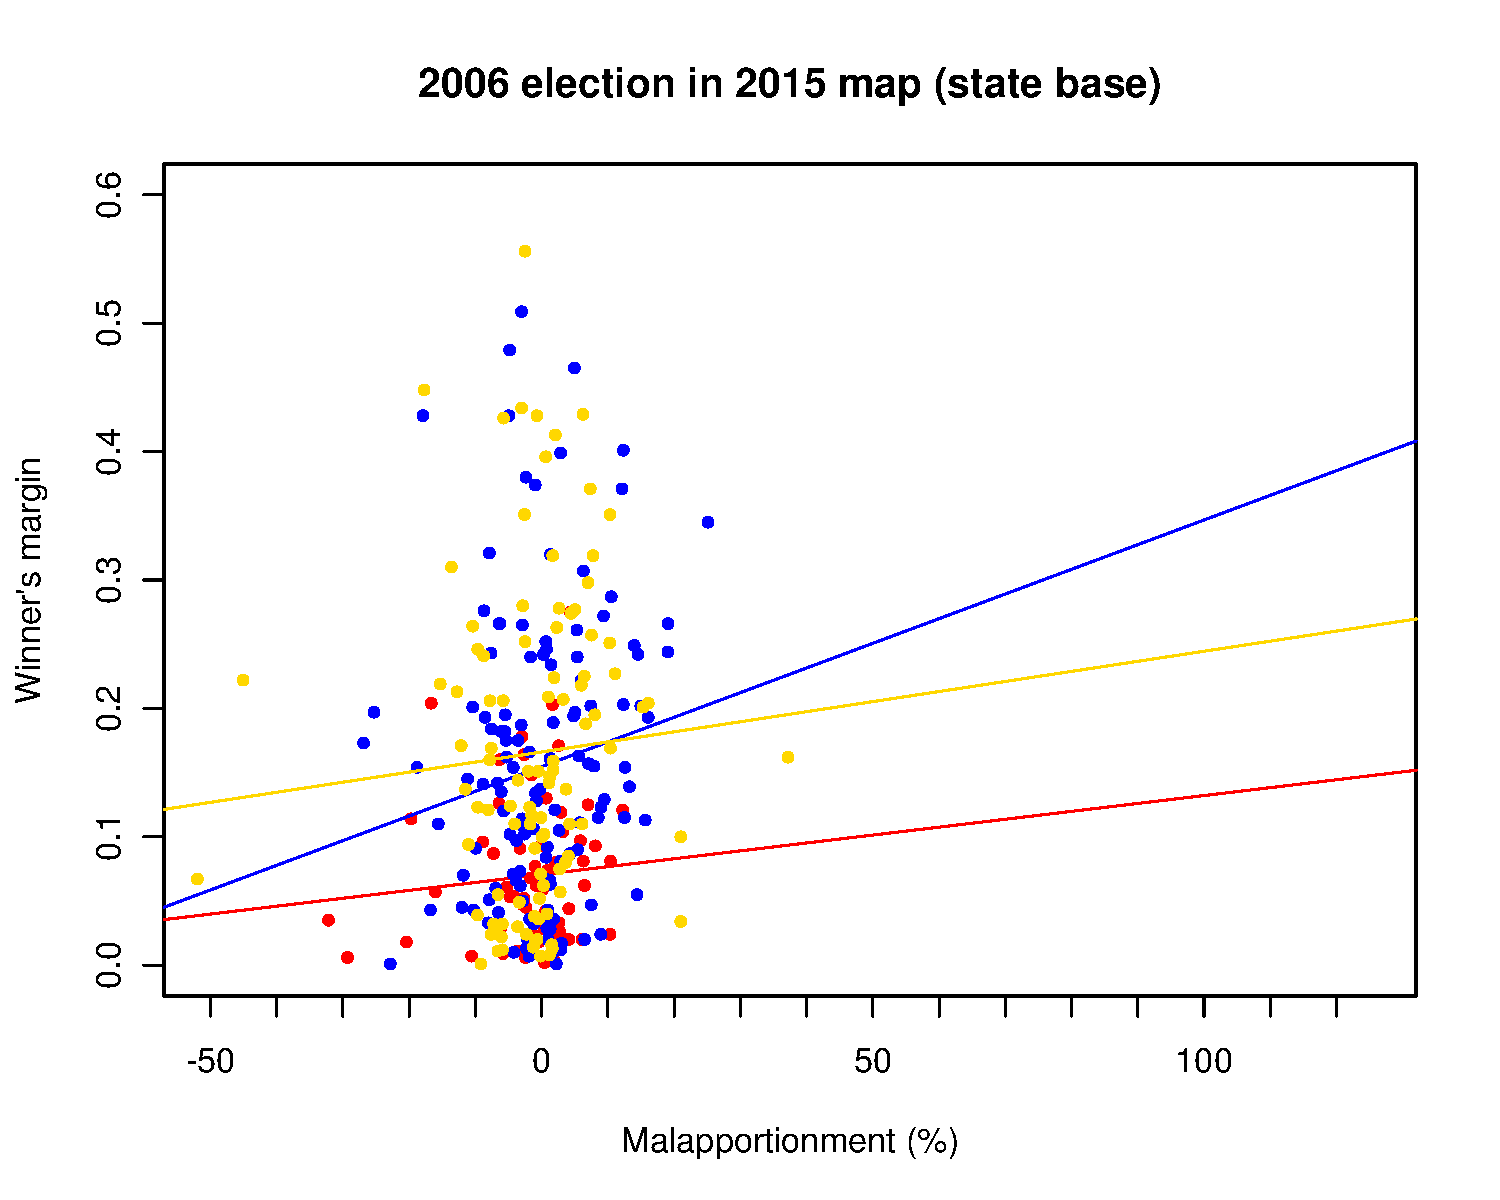
\includegraphics[width=.4\columnwidth]{malmg2006d3sta.pdf} \\
%     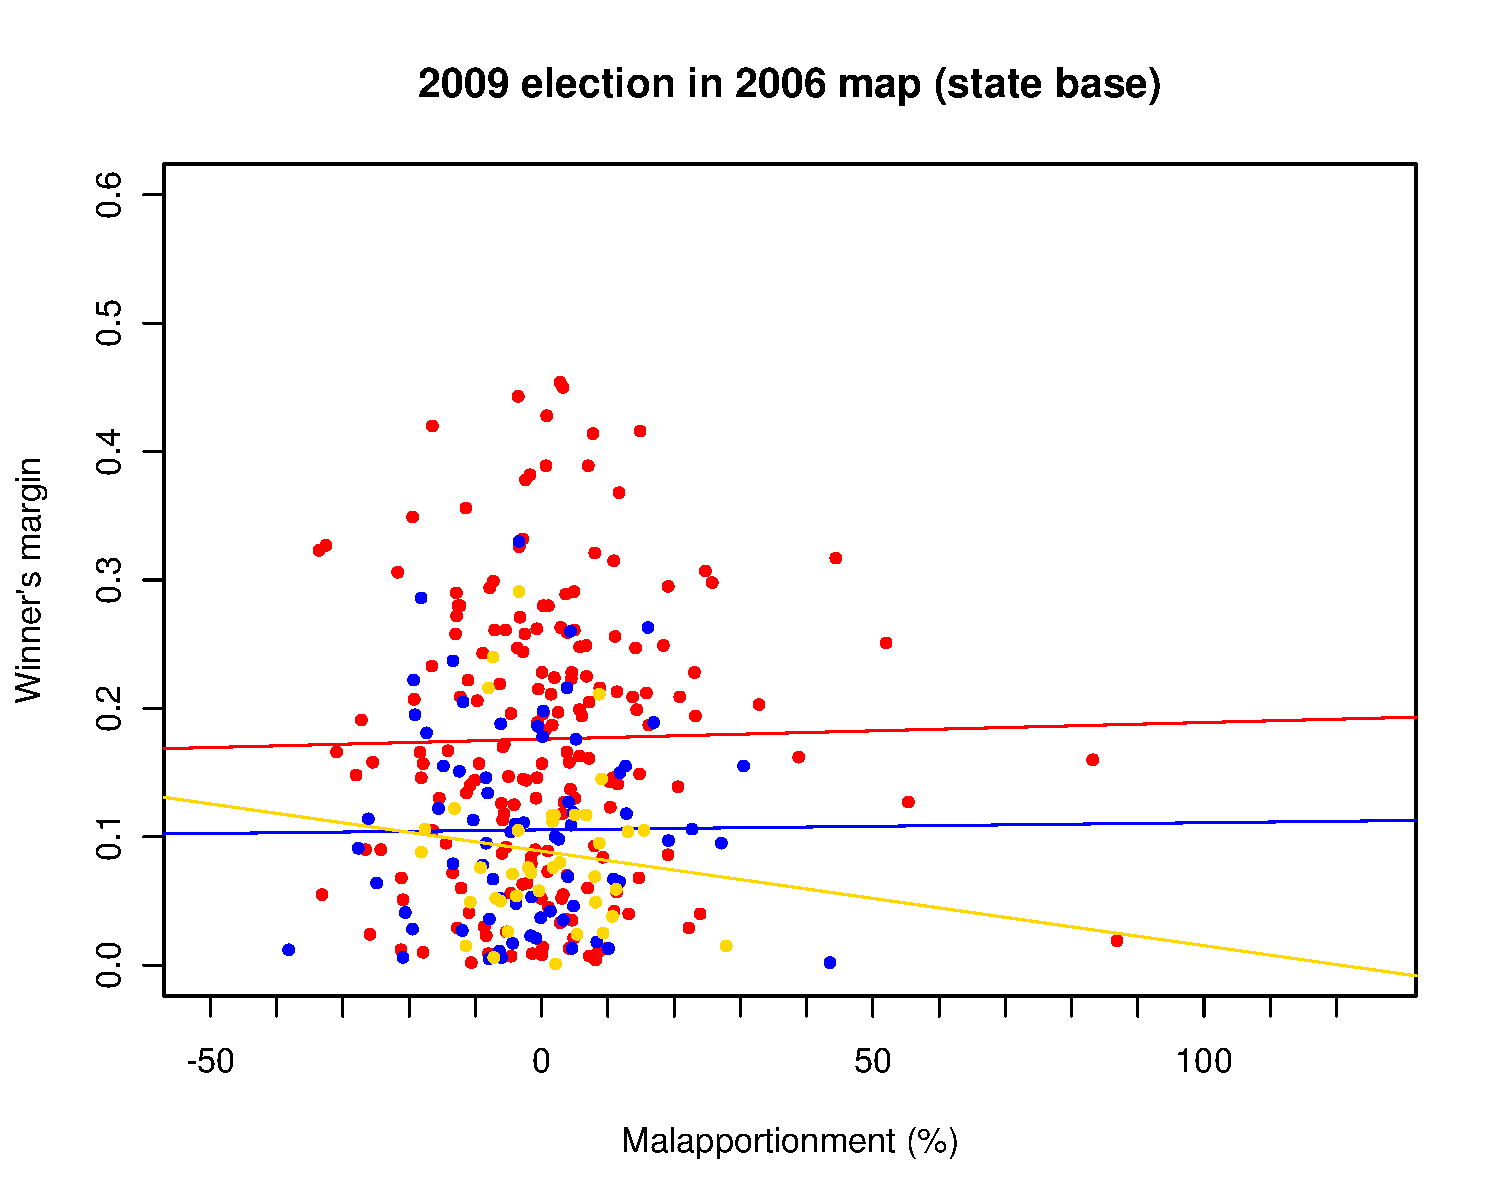
\includegraphics[width=.4\columnwidth]{malmg2009d0sta.pdf} & 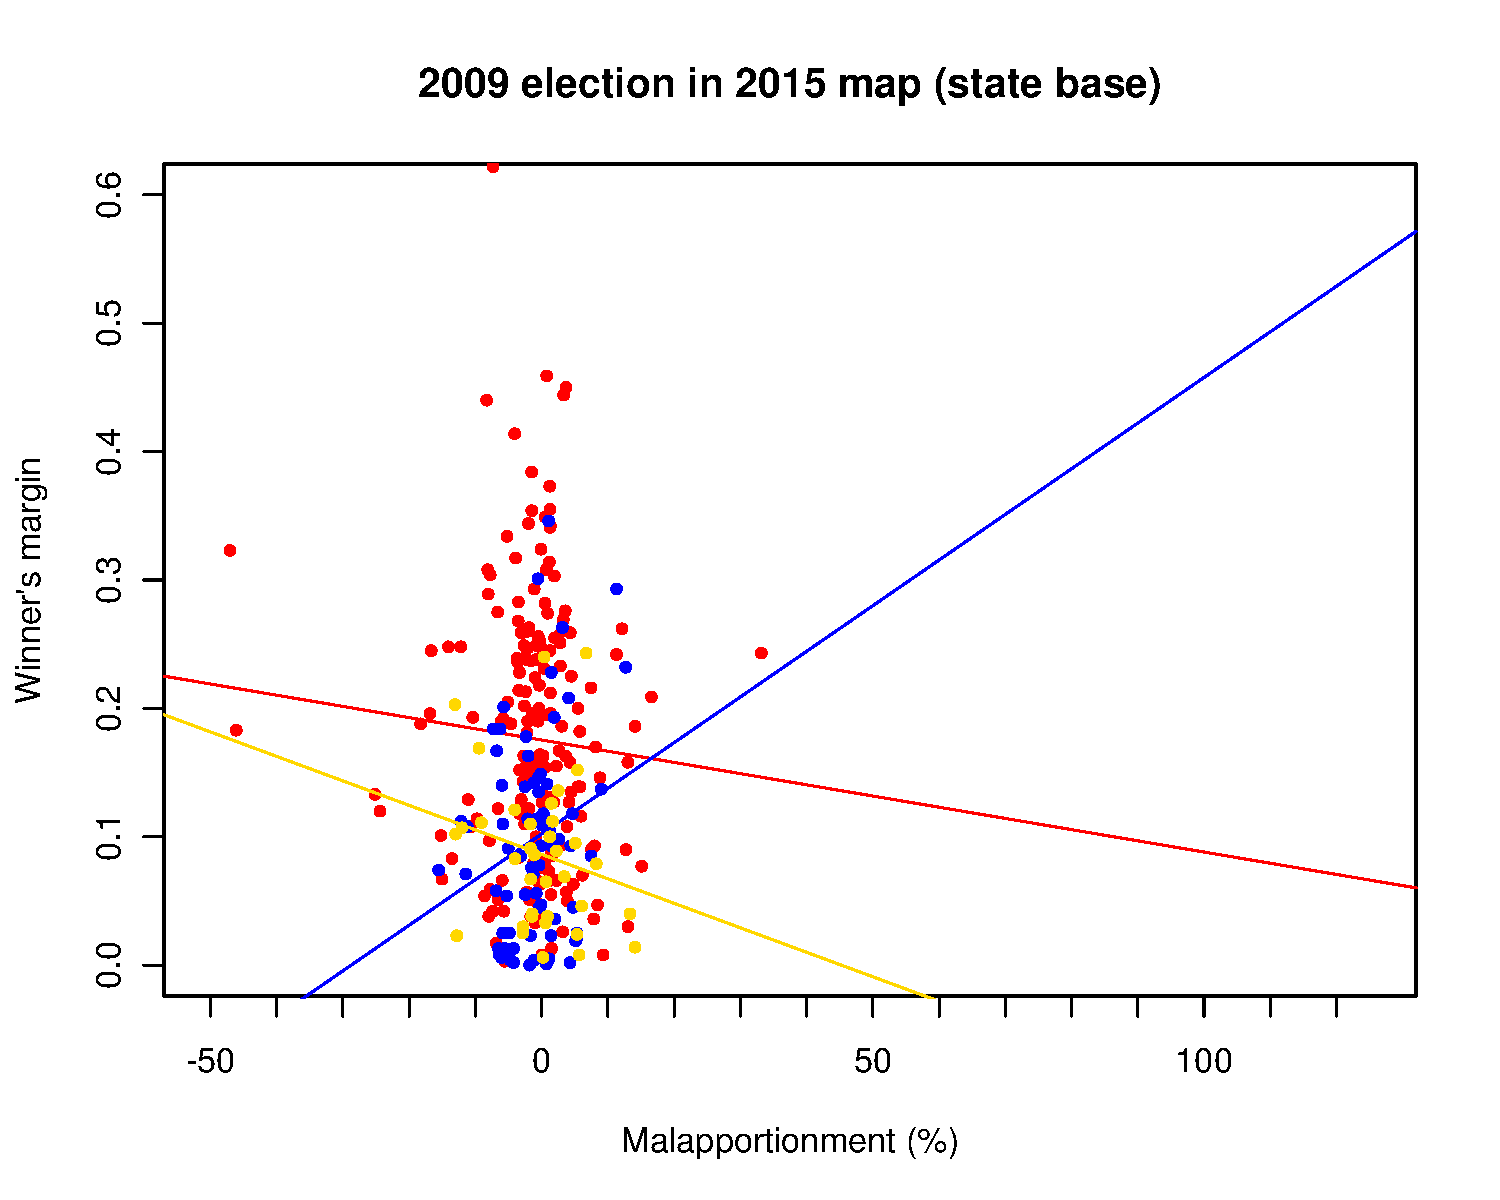
\includegraphics[width=.4\columnwidth]{malmg2009d3sta.pdf} \\
%     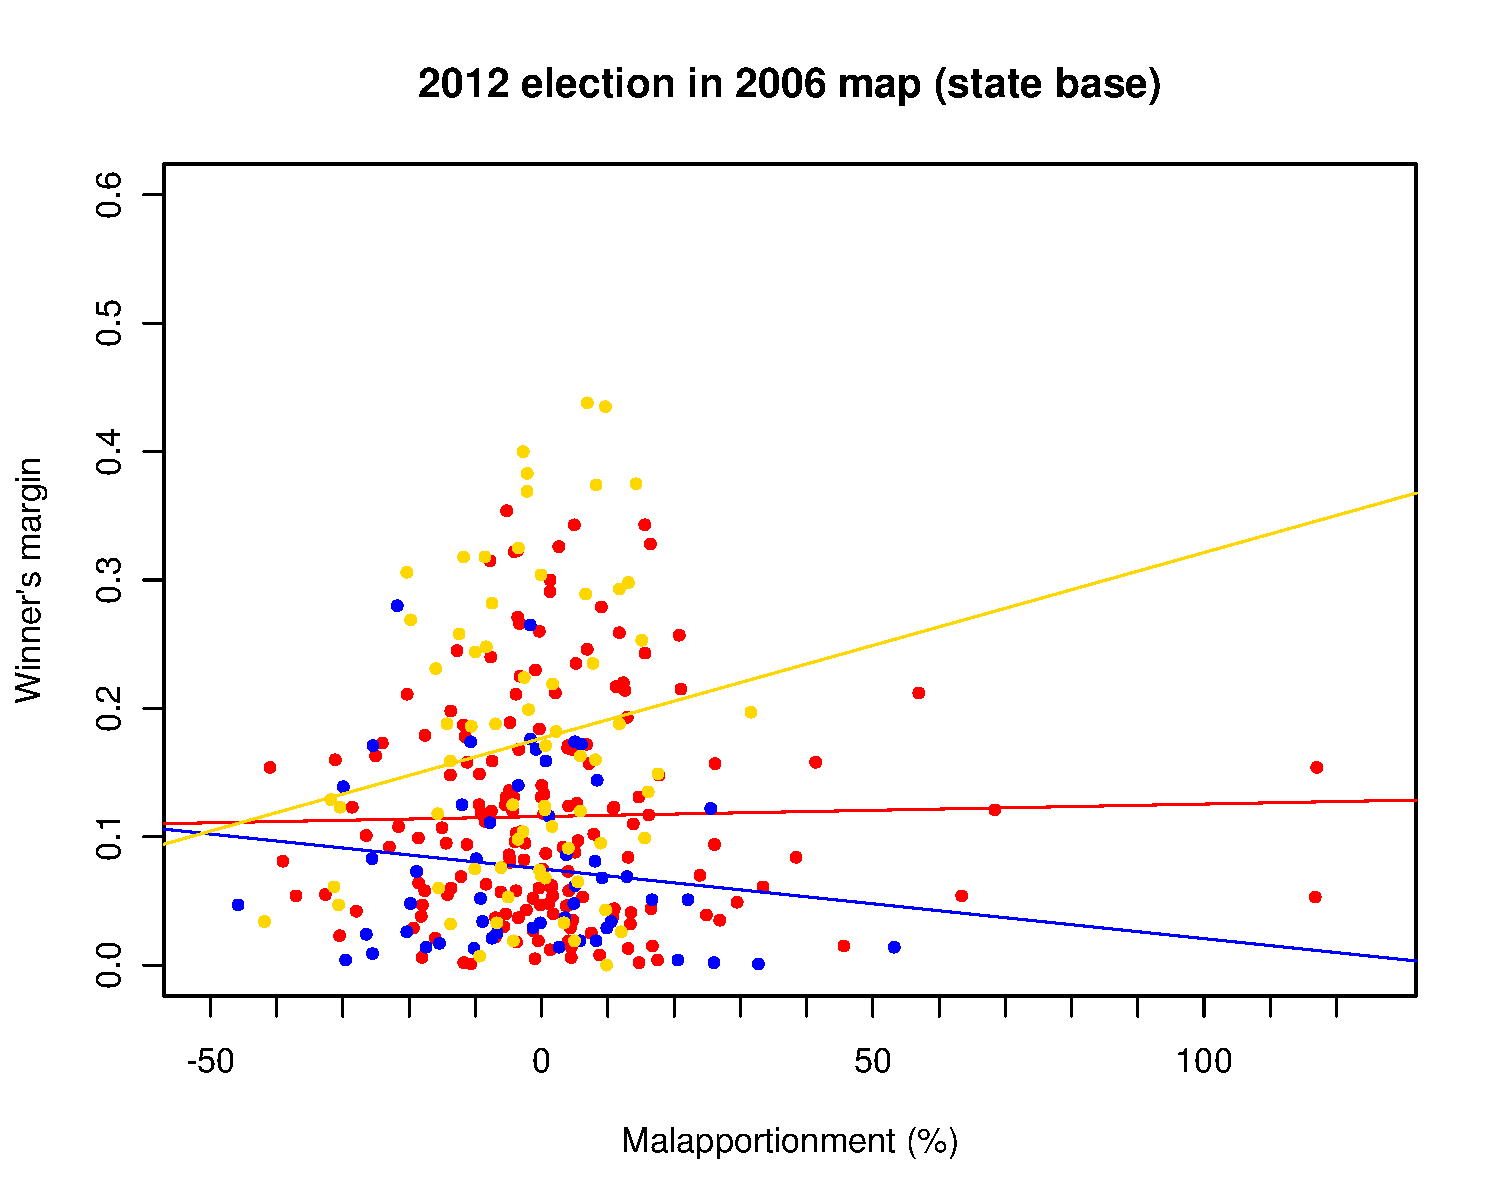
\includegraphics[width=.4\columnwidth]{malmg2012d0sta.pdf} & 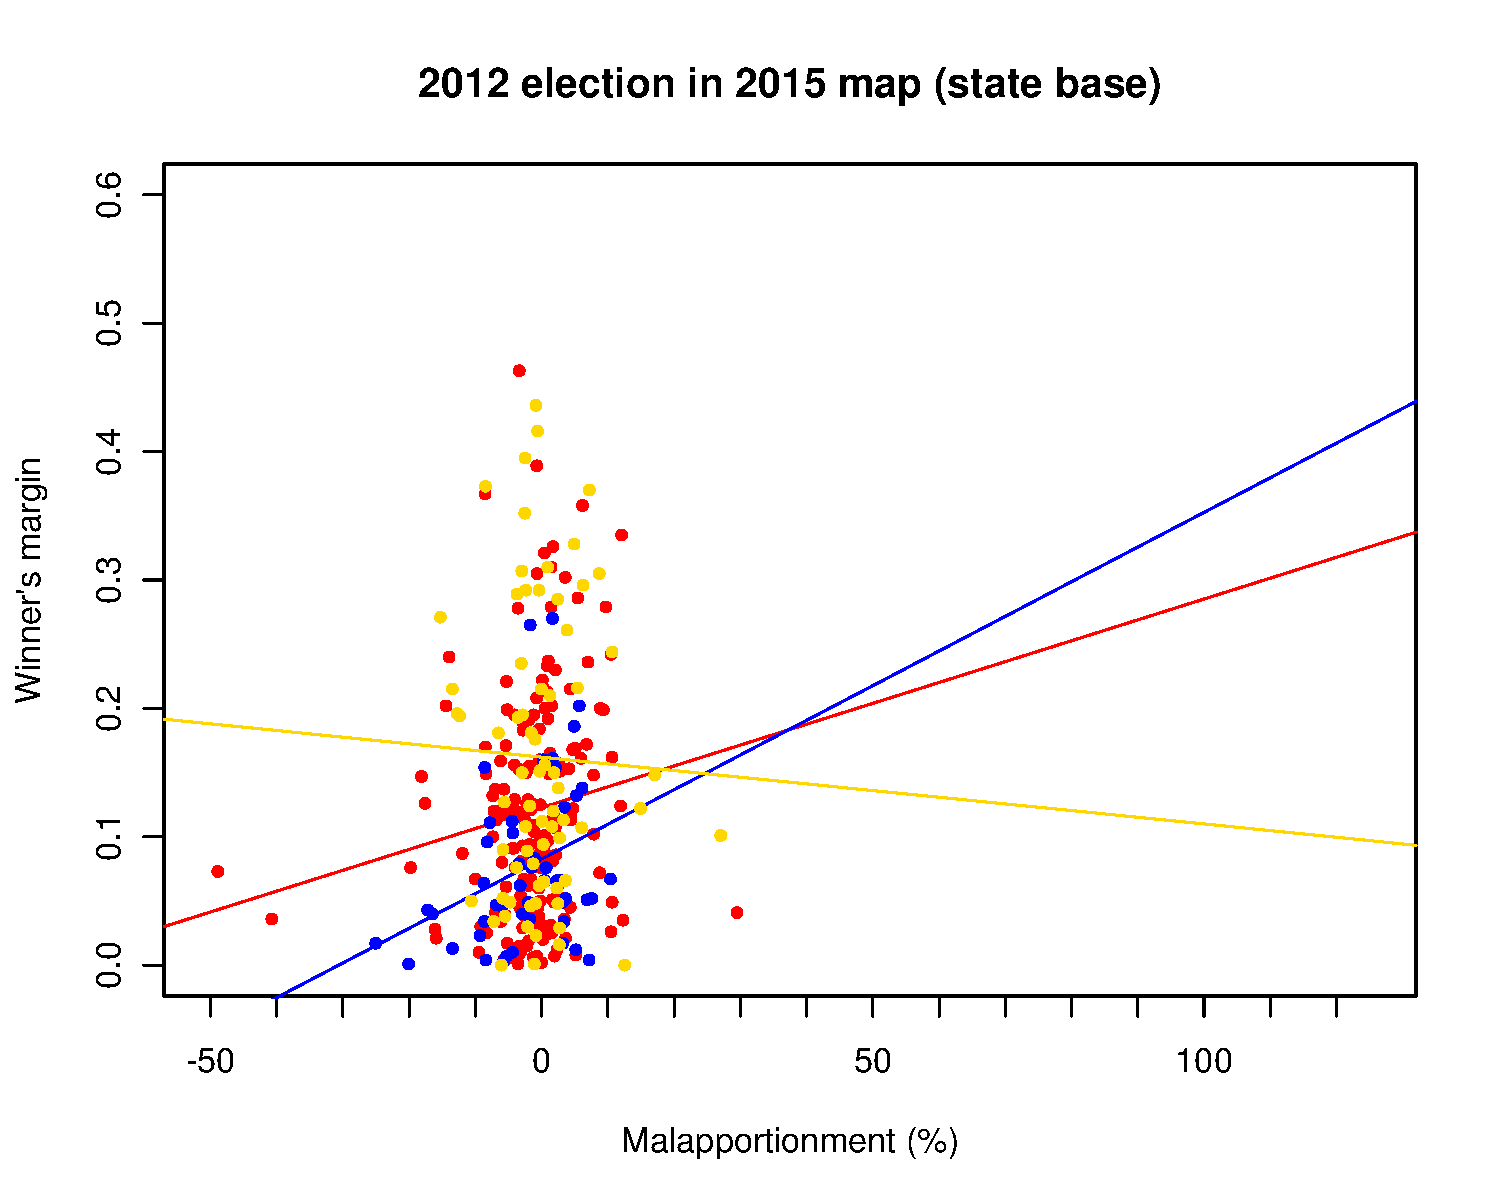
\includegraphics[width=.4\columnwidth]{malmg2012d3sta.pdf} \\
%   \end{tabular}
%   \caption{Vote margin and malapportionment (compared to state averages)}\label{F:malmgsta}
% \end{center}
% \end{figure}

% \begin{figure}
% \begin{center}
%   \begin{tabular}{cc}
%     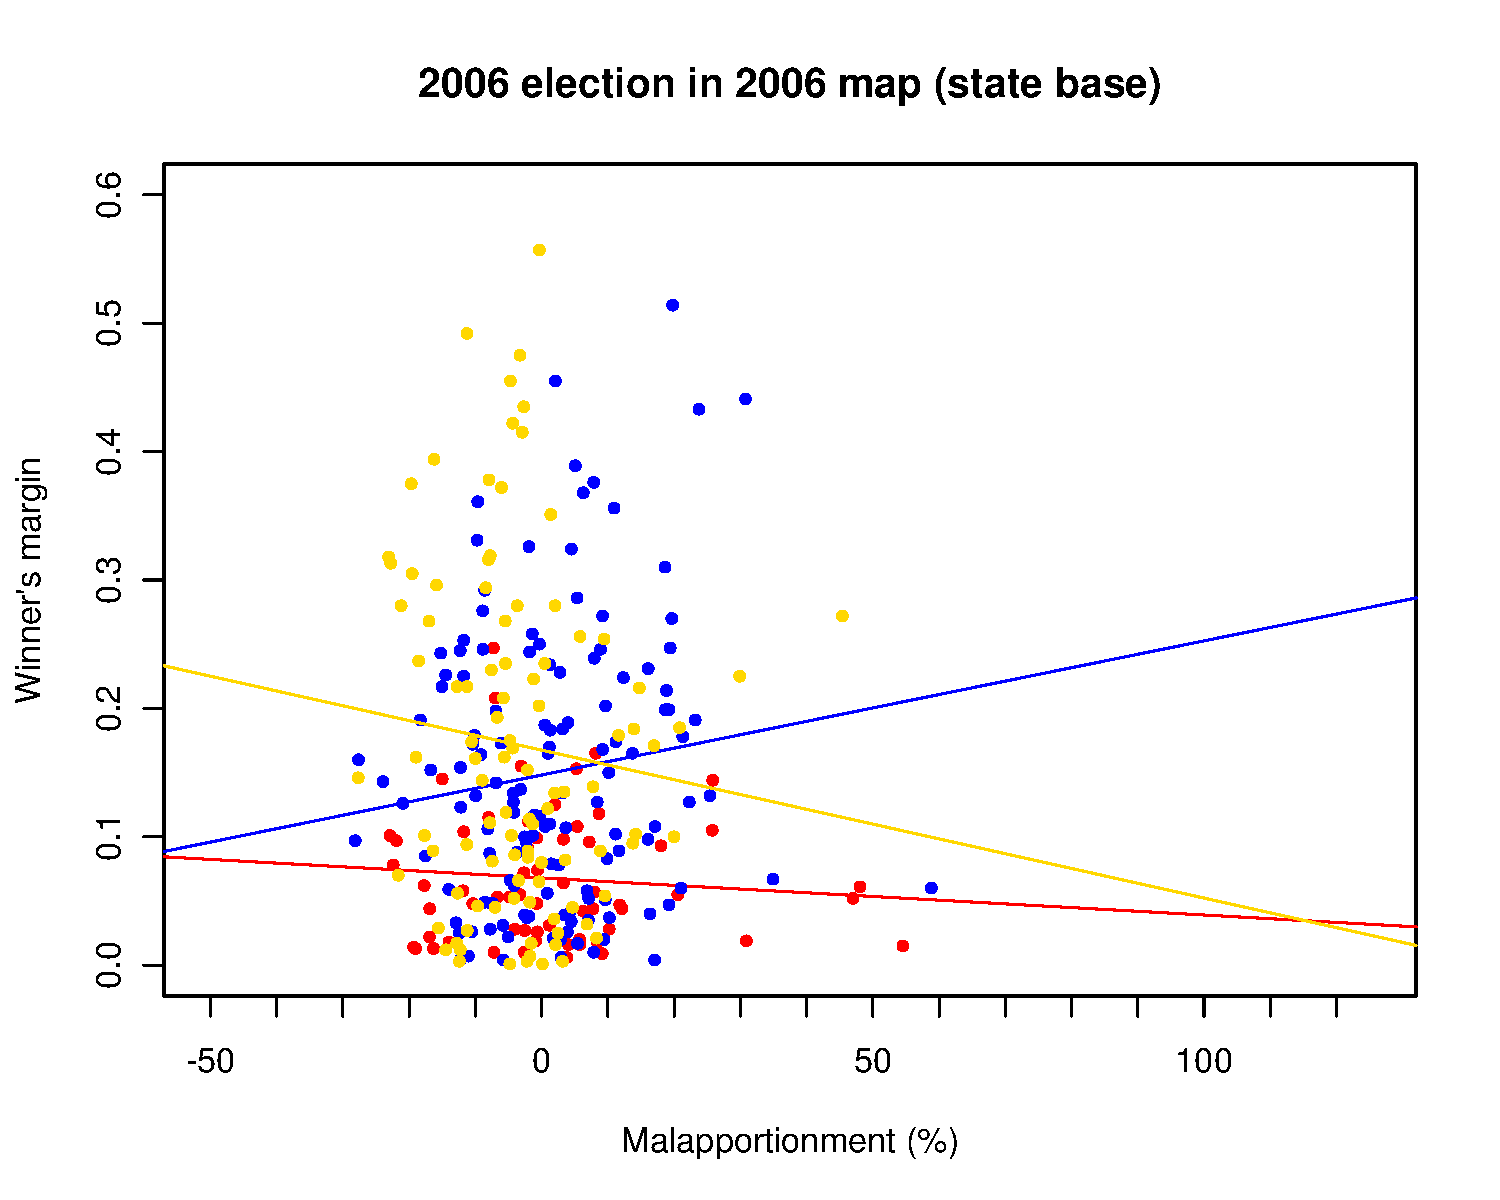
\includegraphics[width=.4\columnwidth]{malmg2006d0nat.pdf} & 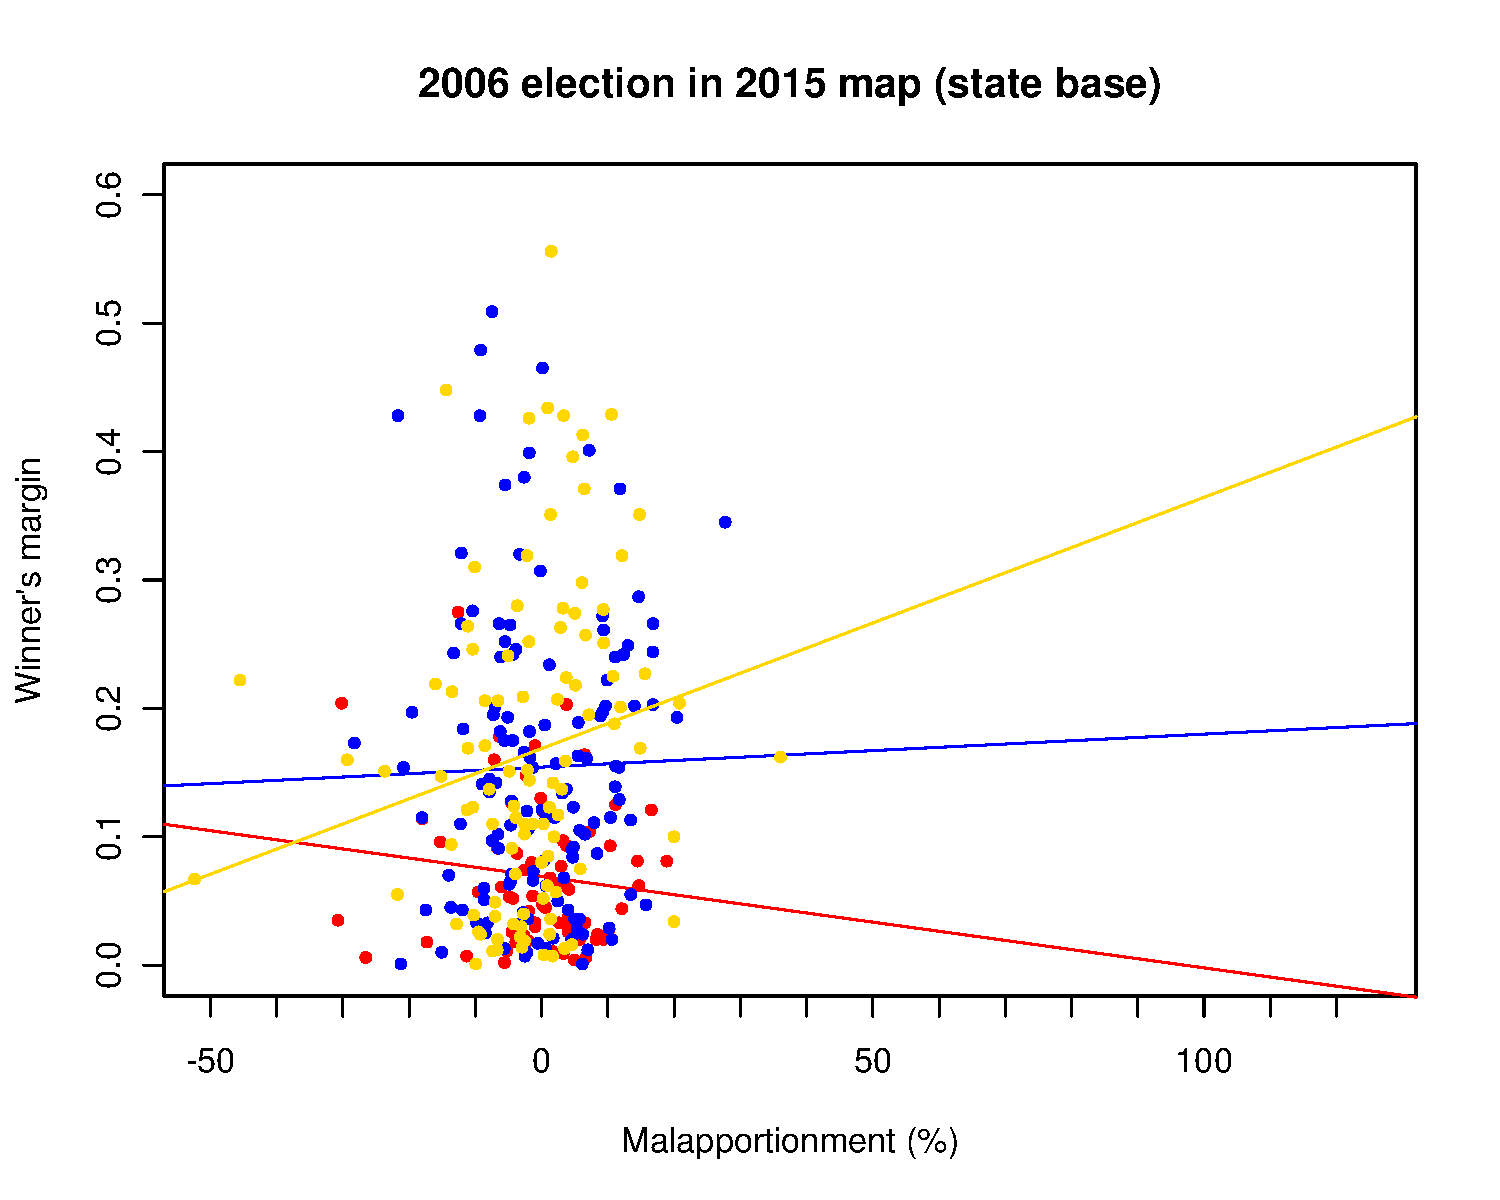
\includegraphics[width=.4\columnwidth]{malmg2006d3nat.pdf} \\
%     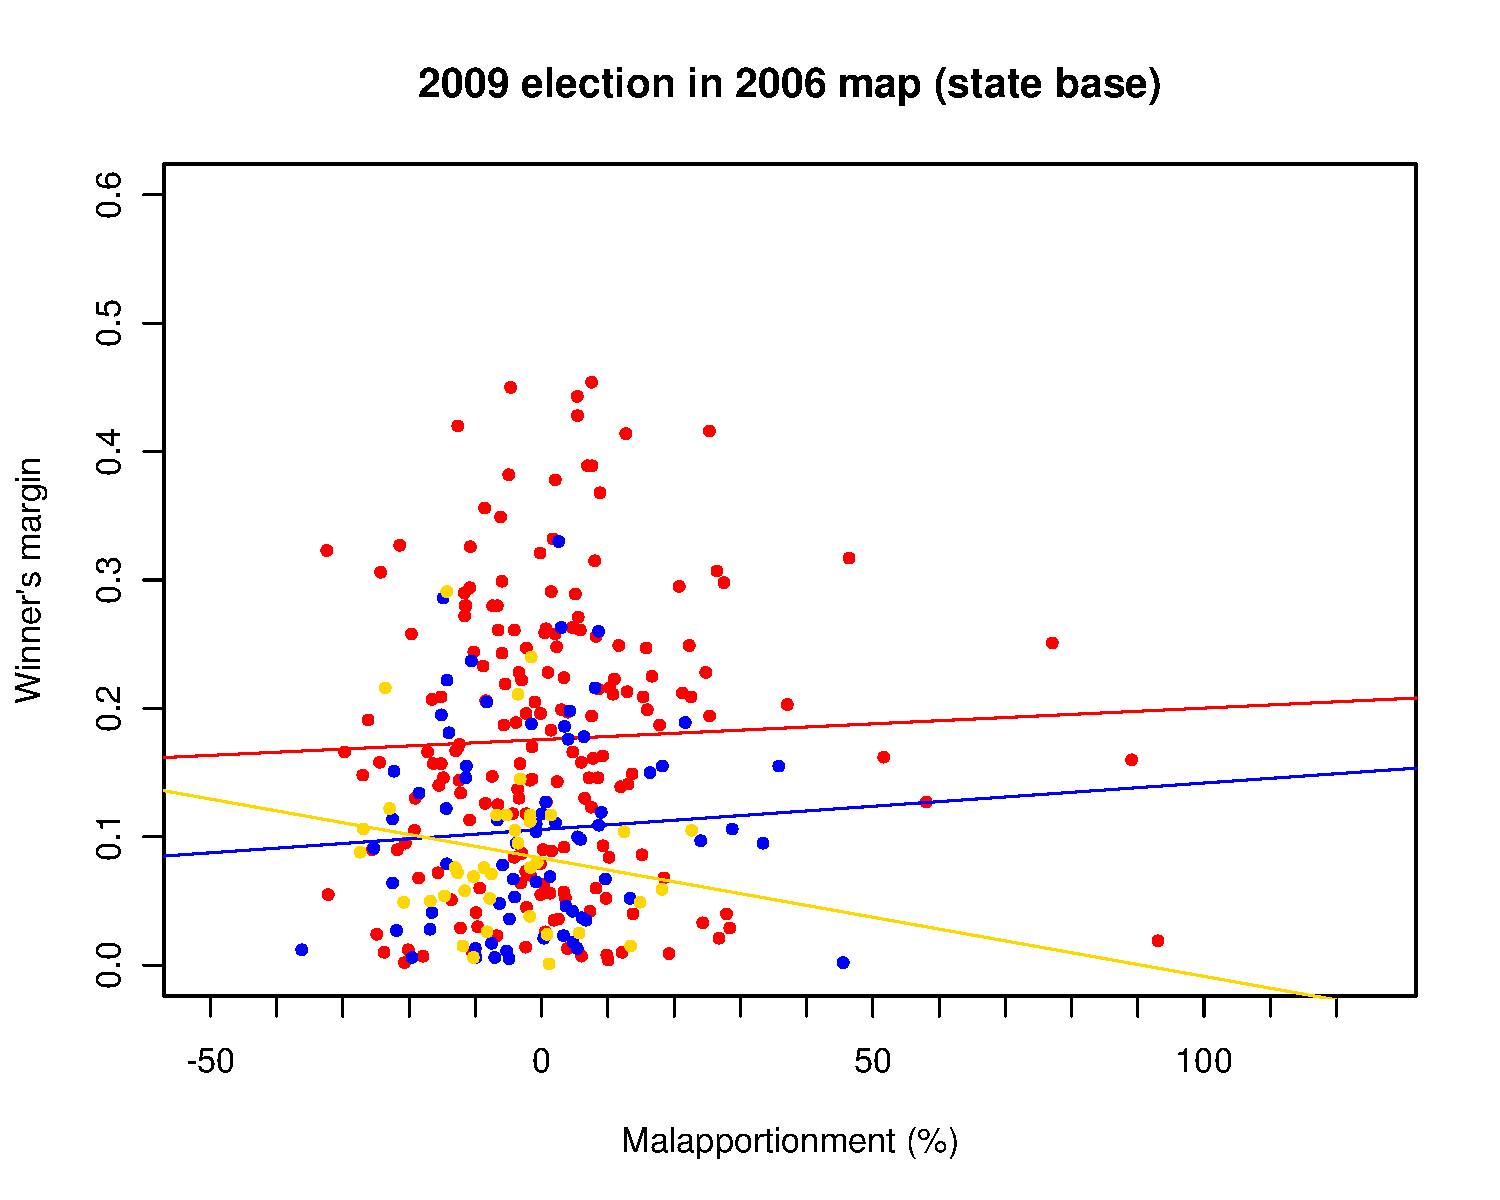
\includegraphics[width=.4\columnwidth]{malmg2009d0nat.pdf} & 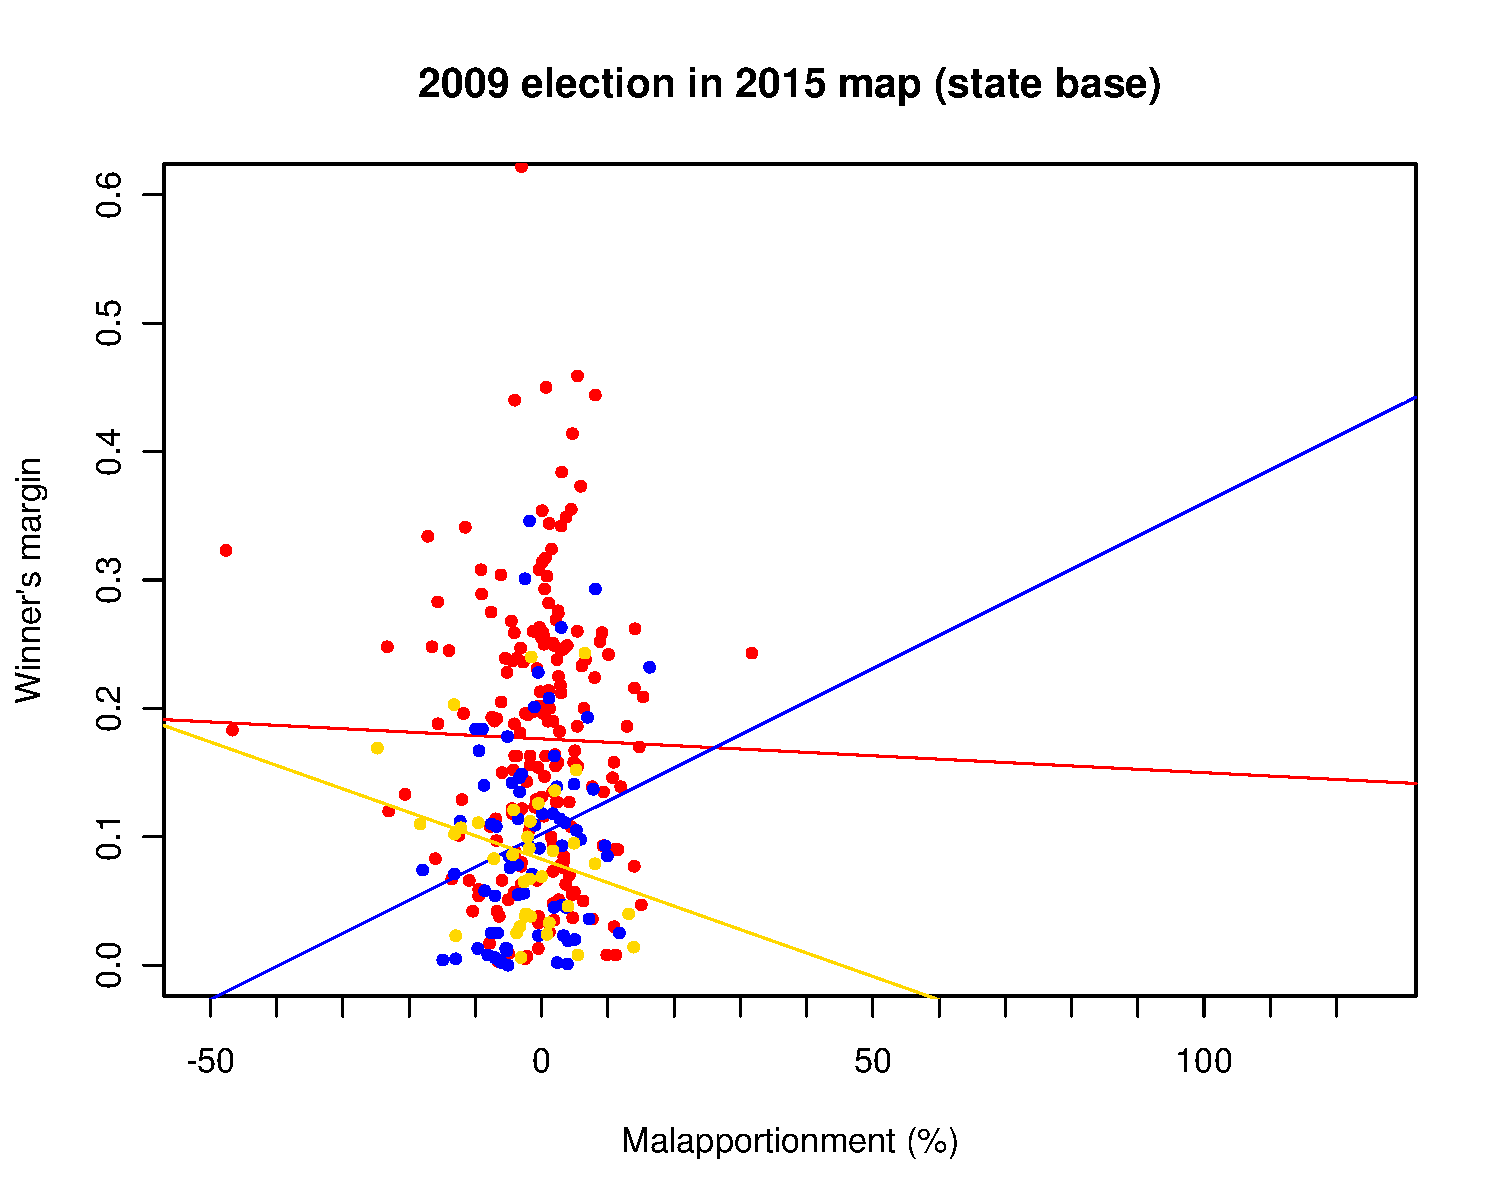
\includegraphics[width=.4\columnwidth]{malmg2009d3nat.pdf} \\
%     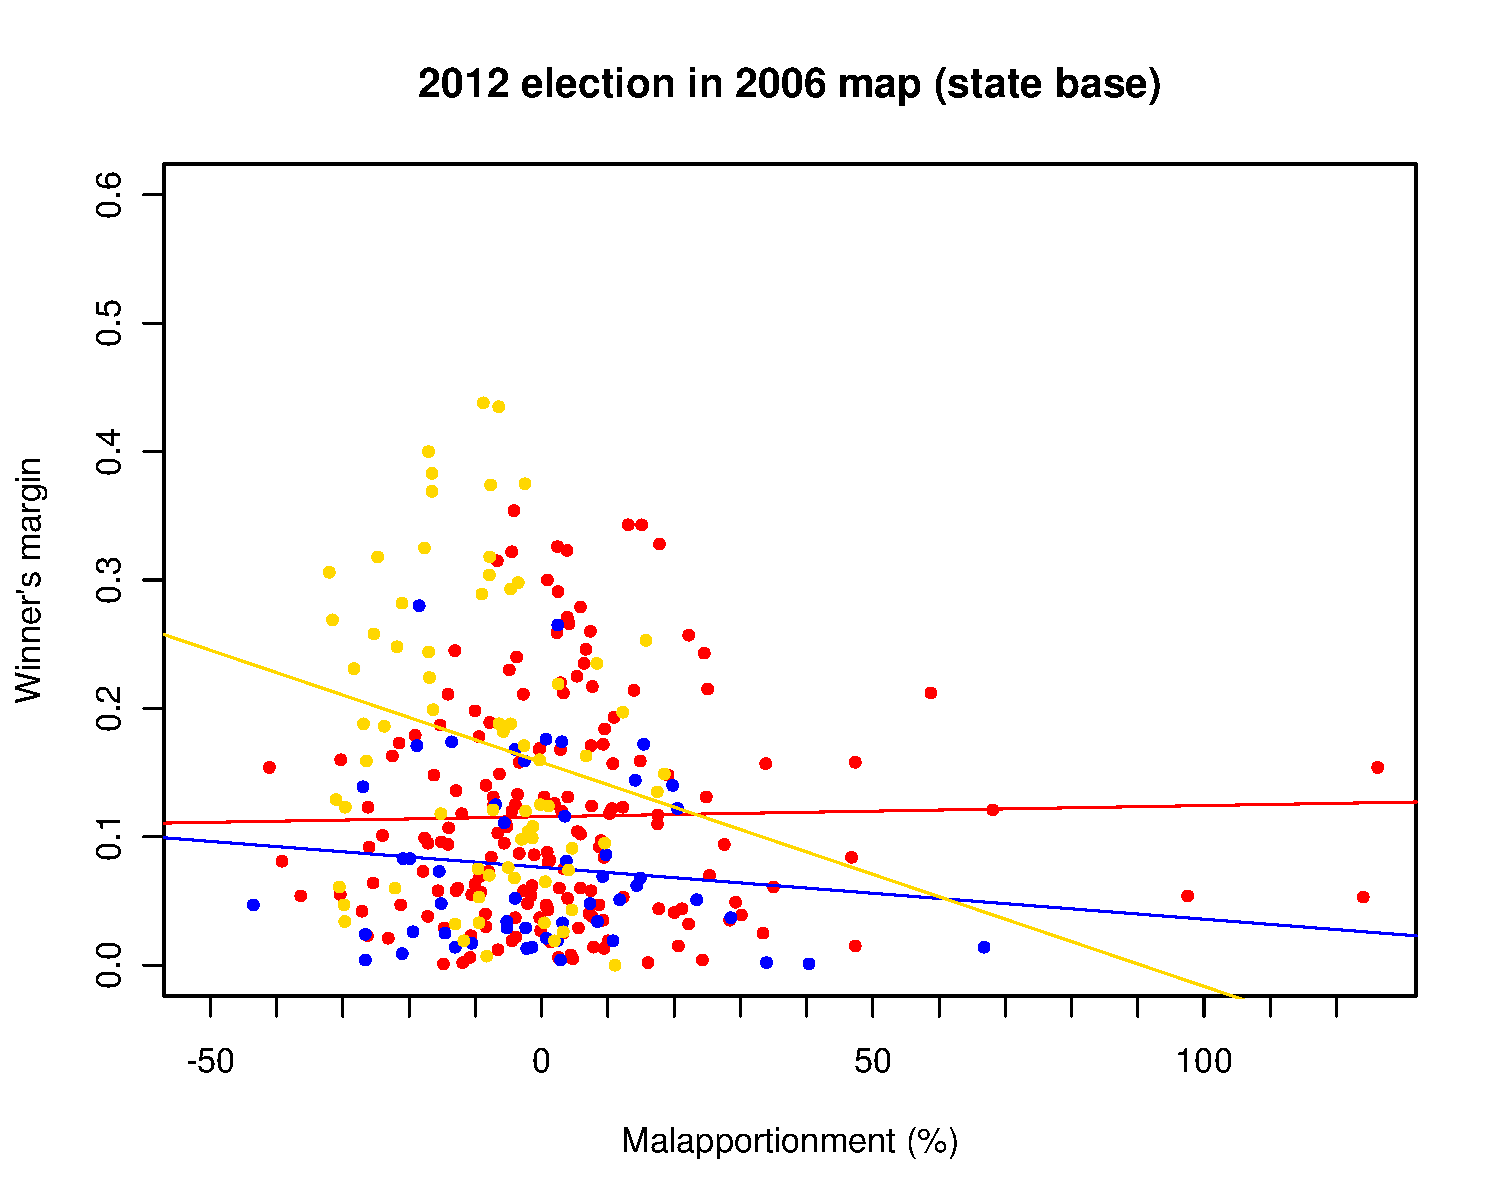
\includegraphics[width=.4\columnwidth]{malmg2012d0nat.pdf} & 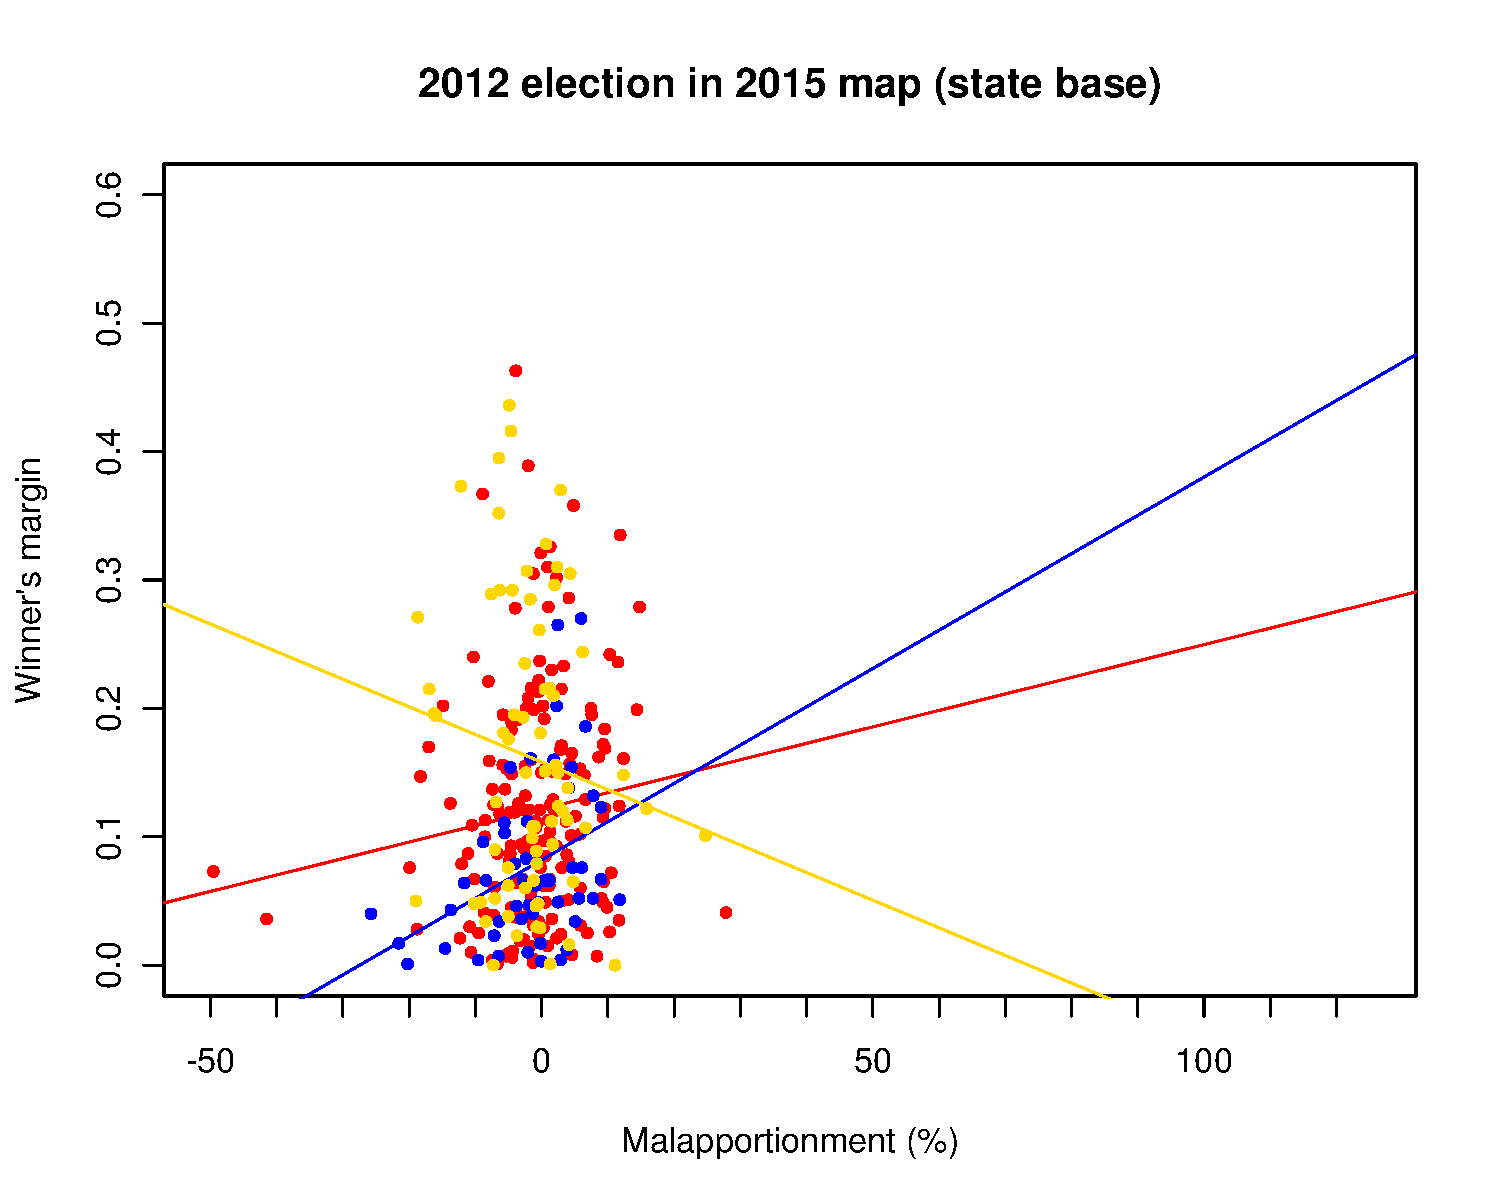
\includegraphics[width=.4\columnwidth]{malmg2012d3nat.pdf} \\
%   \end{tabular}
%   \caption{Vote margin and malapportionment (compared to national average)}\label{F:malmgnat}
% \end{center}
% \end{figure}

% Plots in Figures \ref{F:malmgsta} and \ref{F:malmgnat} 

\section{Conclusion}

** To be written **

Mexico's federal districts exhibit no party bias when analyzed at the state level. Big system responsiveness, typical of first-past-the-post system in units with few federal districts, is associated with the districts. So PRI's tendency to be over-represented more than PAN and PRD, and the PRI's winning of a couple extra seats with the redistricting proposal is not the product of partisan bias. If the PRI wins more this is due to its status as the largest party in more states that the other two major parties combined. 

\section*{Appendix} 

\subsection*{Elasticity}

One district charateristic is how elastic they are to a party's statewide vote (nationwide?). Elasticity should shape redistricting preferences. A district is highly elastic for the PAN when small shifts in the party's vote statewide correspond to sharp district vote hikes. It is inelastic when it corresponds to more modest district vote changes. Negative elasticity is even conceivable, the district vote growing when the rest of the state shrinks. Local effects on mobilization and voting can move against state effects. If every section in the district is a microcosm of the state's electorate, unit elasticity ensues. 

The measure regresses a party's three-year vote change in the section $\Delta_s$ on the the parent state vote change $\Delta_e$ thus:  

\begin{equation}
\Delta_s = \sum\limits_{d=1}^{D_e} \alpha_d + \beta_d \Delta_e.
\end{equation}

\noindent Fixed effects for each district are considered, fitting separate $\alpha_d$ and $\beta_d$ regression coefficients for every district (indexed $d$). The model is estimated for every state separately because doing it nationwide involves too many sections (67k) and parameters (600) for my machine. 

\begin{figure}
\begin{center}
  \begin{tabular}{cc}
    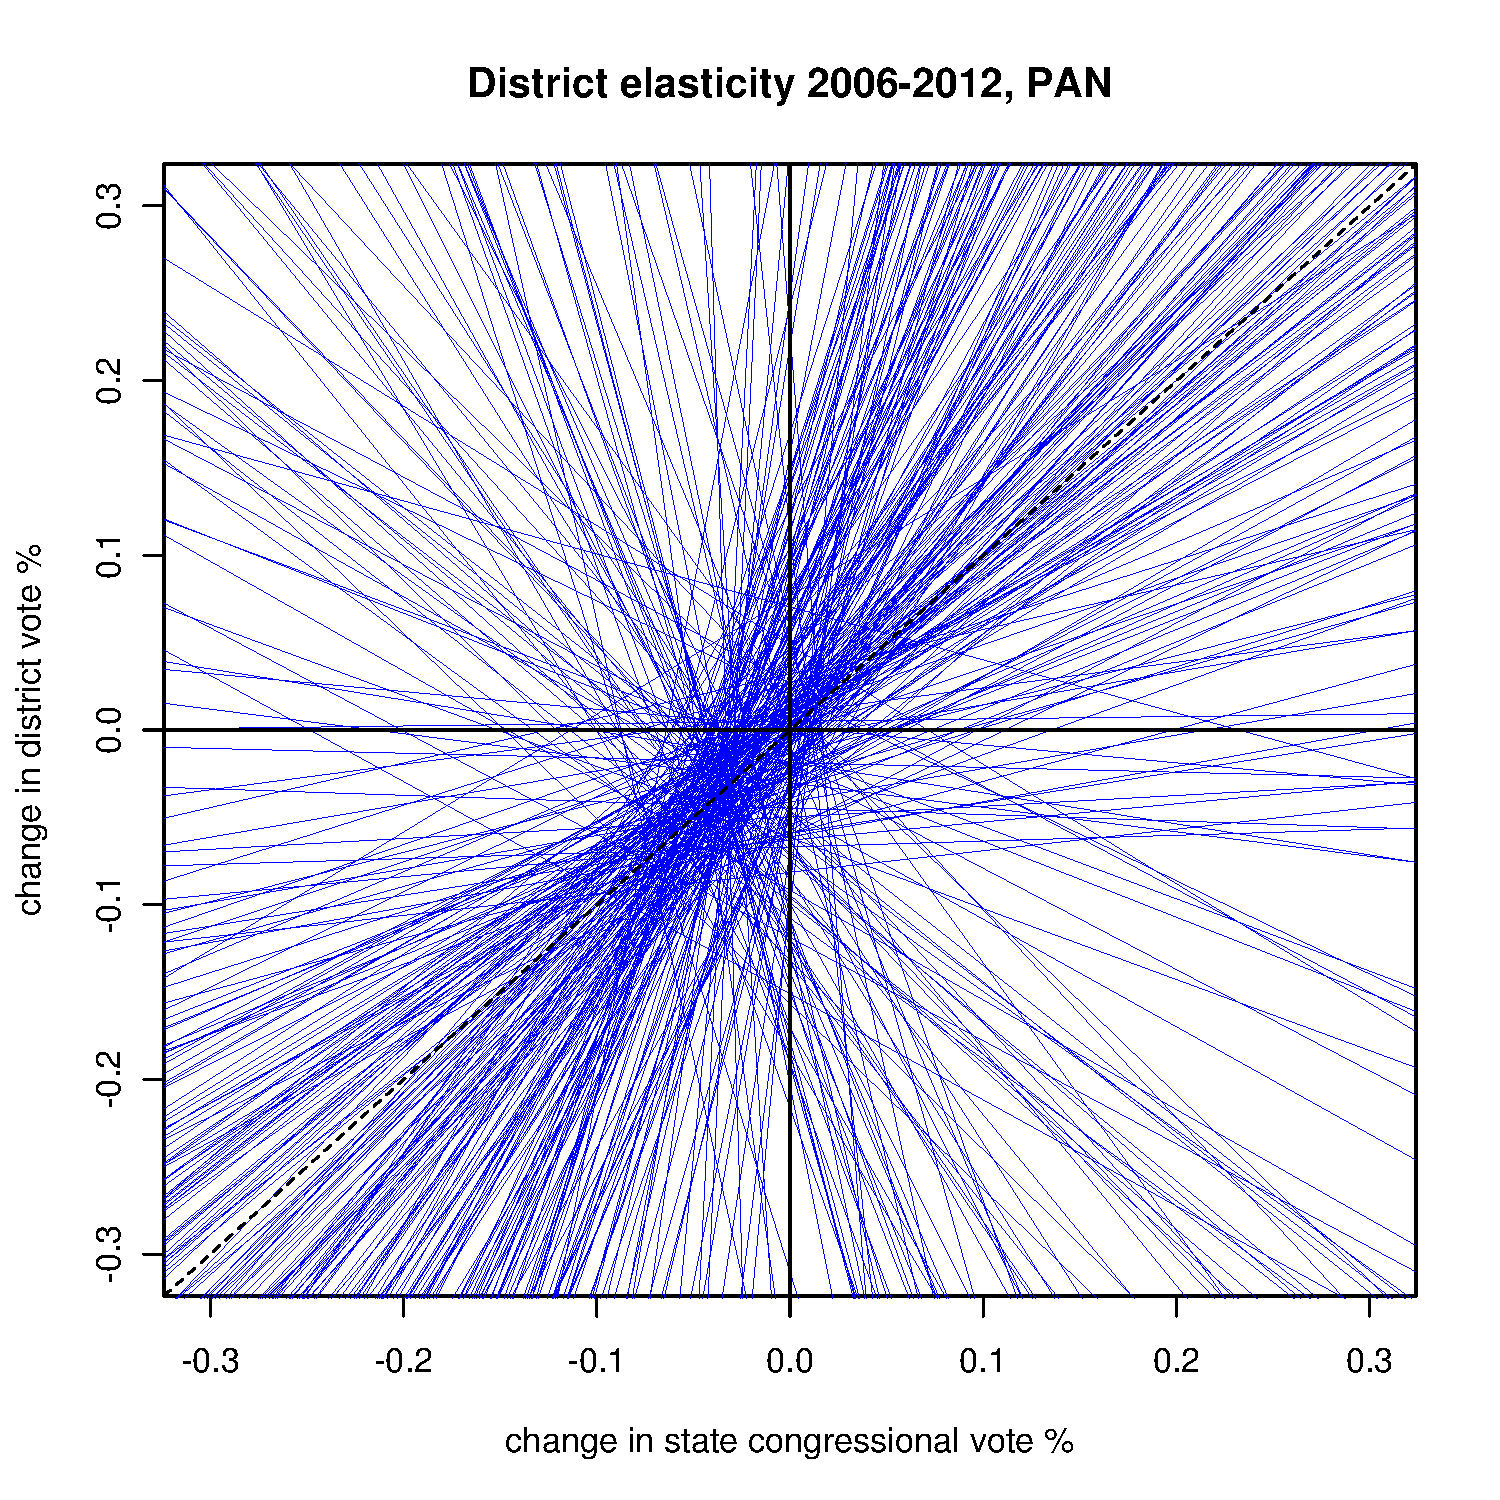
\includegraphics[width=.4\columnwidth]{elastpand0.pdf} & 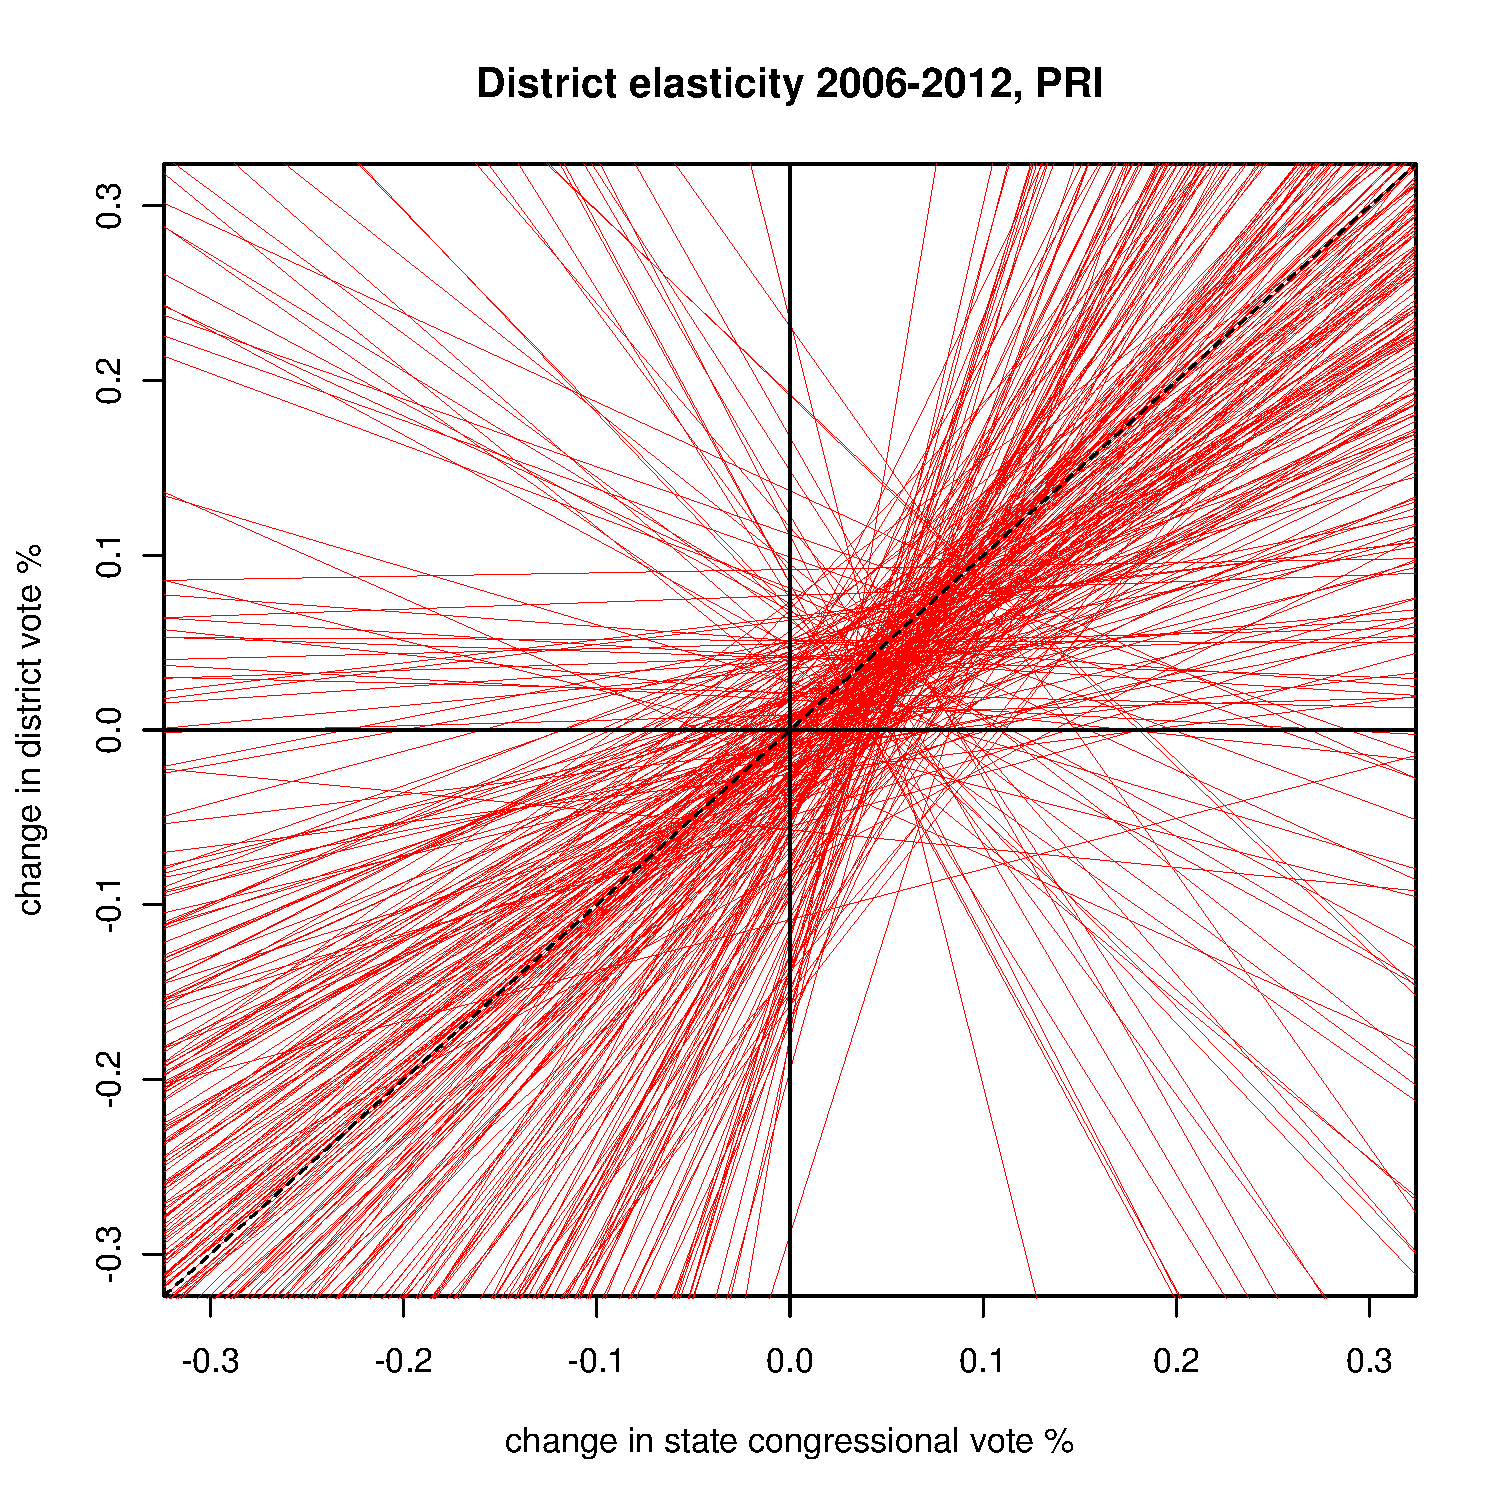
\includegraphics[width=.4\columnwidth]{elastprid0.pdf} \\
    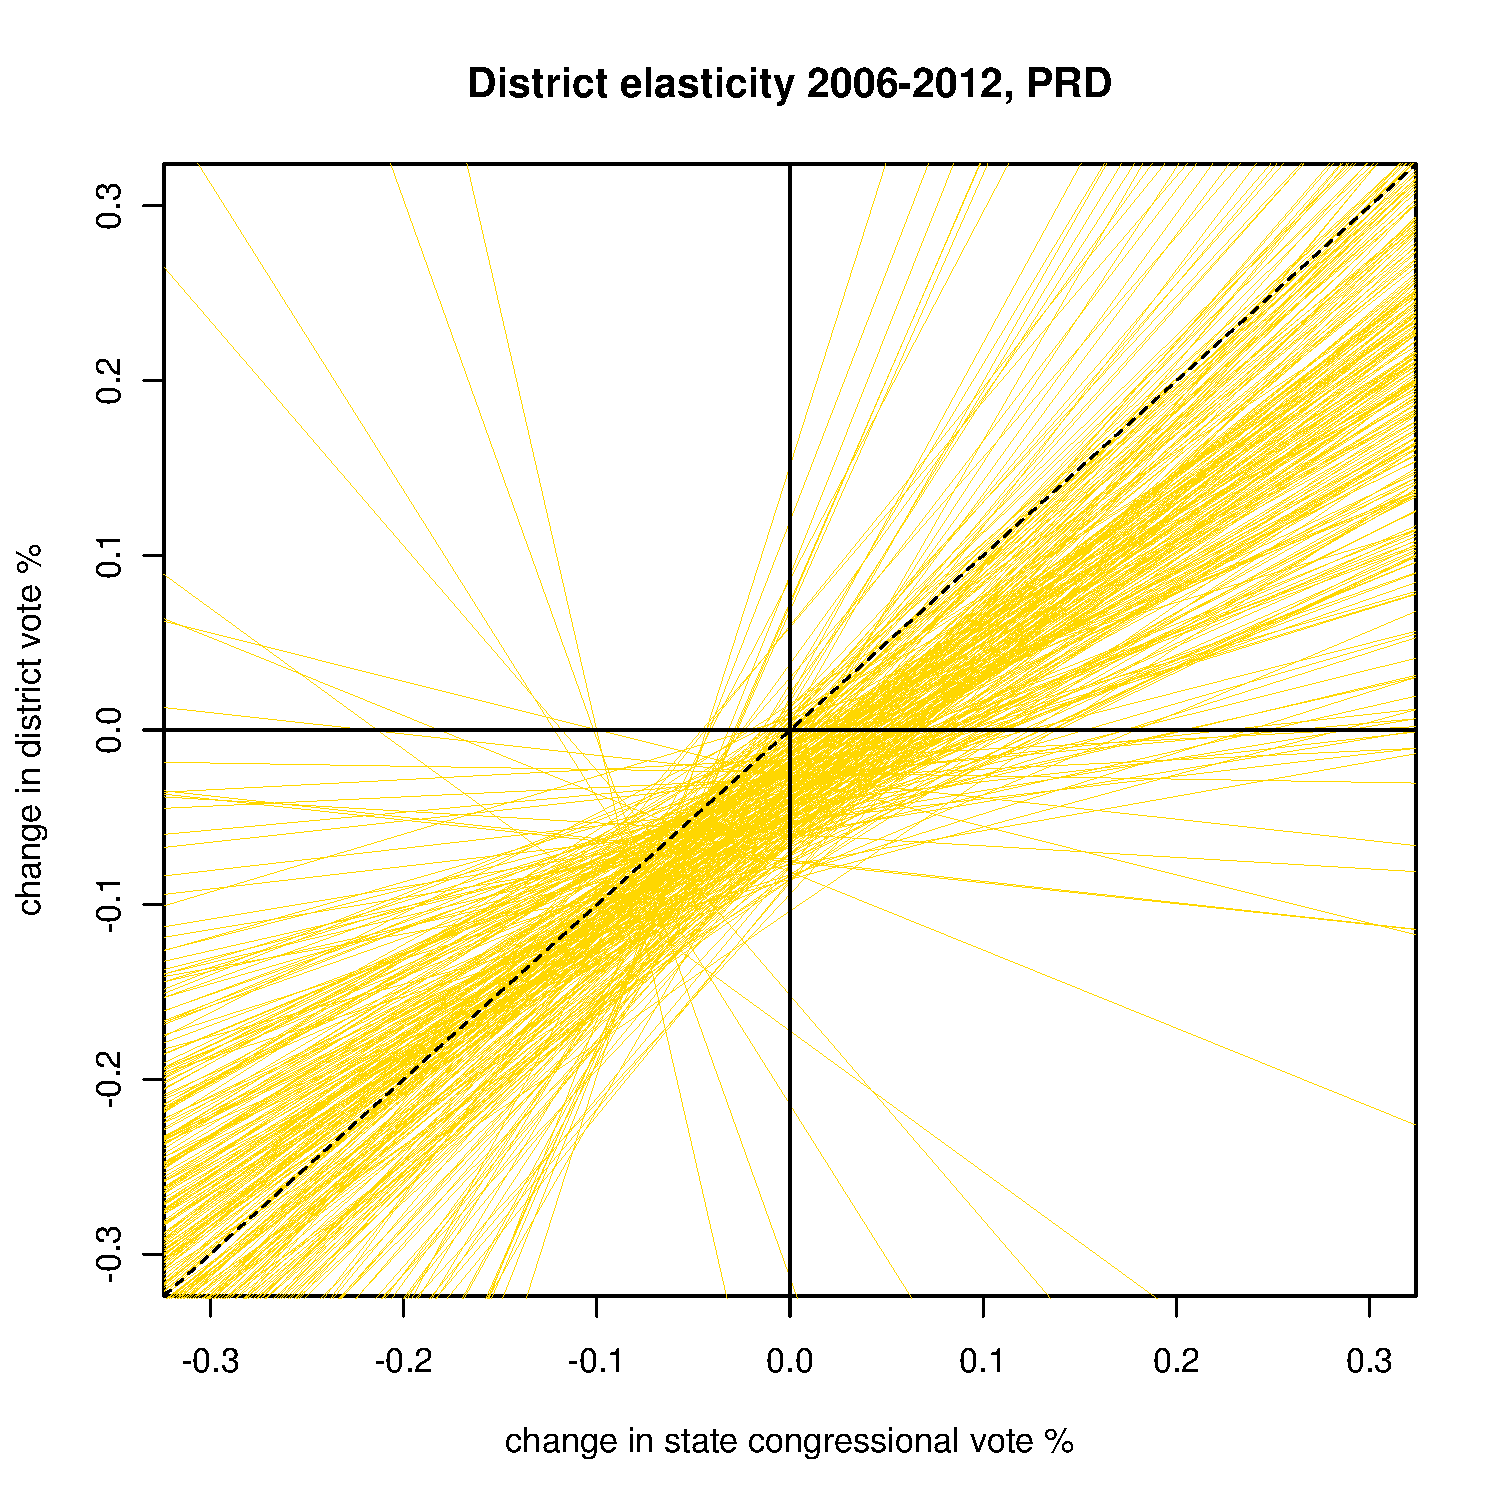
\includegraphics[width=.4\columnwidth]{elastprdd0.pdf} &  \\
  \end{tabular}
  \caption{Parties' district elasticities}\label{F:malmgnat}
\end{center}
\end{figure}


%sensitive of insulated they are from the party's fate in the state. The measure is associated to the party record \citep{cox.mccubbins.1993}, ``a commonly accepted summary of the past actions, beliefs, and outcomes with which [the party] is associated'' (102). Cox and McCubbins focus on national parties, but recognize that the party record varies from state to state (whose voters focus on different elements of the record). The measure here is how, and how much change in the district vote relates to the statewide change in a party's congressional vote. If every section in the district were a microcosm of the state's electorate, a one-on-one relation would ensue -- a 5 percent drop in the state corresponds to a 5 percent drop in the district. If the party's vote drops less, or even holds or improves, in many of the district's sections, the party performs relatively better (or less badly) in the district. District responsiveness to or insulation from the state party vote may be valuable in different circumstances. 



\bibliographystyle{apsr}
\bibliography{../../../../../mydocs/magar}
%\bibliography{bib/magar}


\end{document}
